\documentclass[a4paper]{article}

\usepackage{ReportTemplate}

\usepackage{setspace}
\usepackage{amsmath}
\usepackage[hidelinks]{hyperref}
\usepackage{float}
\usepackage{algorithm}
\usepackage{algpseudocode}
\usepackage{booktabs}
\usepackage{svg}




\title{Project 1:语音端点检测}
\name{杨炫锟}
\studentid{523030910248}

\begin{document}

\maketitle

\section{基于线性分类器和语音短时能量的简单语音端点检测算法}

\subsection{数据预处理及特征提取}

\begin{itemize}
  \item 
  {
    在任务一中,我使用的预处理方法有:
    \begin{itemize}
      \item \textbf{预加重处理}
      \item \textbf{分帧}
      \item \textbf{短时傅里叶变换前的加窗}
    \end{itemize}
  }
  \item 
  {
    在任务一中,我提取的语音特征有:
    \begin{itemize}
      \item \textbf{短时能量}
      \item \textbf{短时过零率}
      \item \textbf{短时基频}
      \item \textbf{短时频谱均值}
      \item \textbf{短时子带能量}
    \end{itemize}
  }
  \end{itemize}
  

\subsubsection{预加重处理}

\begin{enumerate}
  \item 
  {
    目的:

    在一个频段范围内,用来增加某一些频率的幅值(一般是较高的频率)w.r.t.
    降低另一些频率的幅值(一般是较低的频率),从而增强信号整体的信噪比。
  }
  \item 
  {
    计算:

    具体计算如式\ref{eq:pre_emphasis}
    \begin{equation}
      x_n = x_n - \alpha x_{n-1}
      \label{eq:pre_emphasis}
    \end{equation}
  }
  \item 
  {
    效果:

    为更加直观地观察预加重处理对数据的影响,我选取了开发集中的一段语音信号,
    取出其中帧长为$512$的一帧信号(这里只是为了让数据更直观,原始处理应该是对整段语音信号进行处理),
    分别做了以下操作:不进行预加重处理,进行预加重处理,并设置$\alpha$分别为$0.5, 0.9, 1.0$,
    并作出对应得到的语音的波形与幅度谱,得到如下效果图:
    \begin{figure}[H]
      \centering
      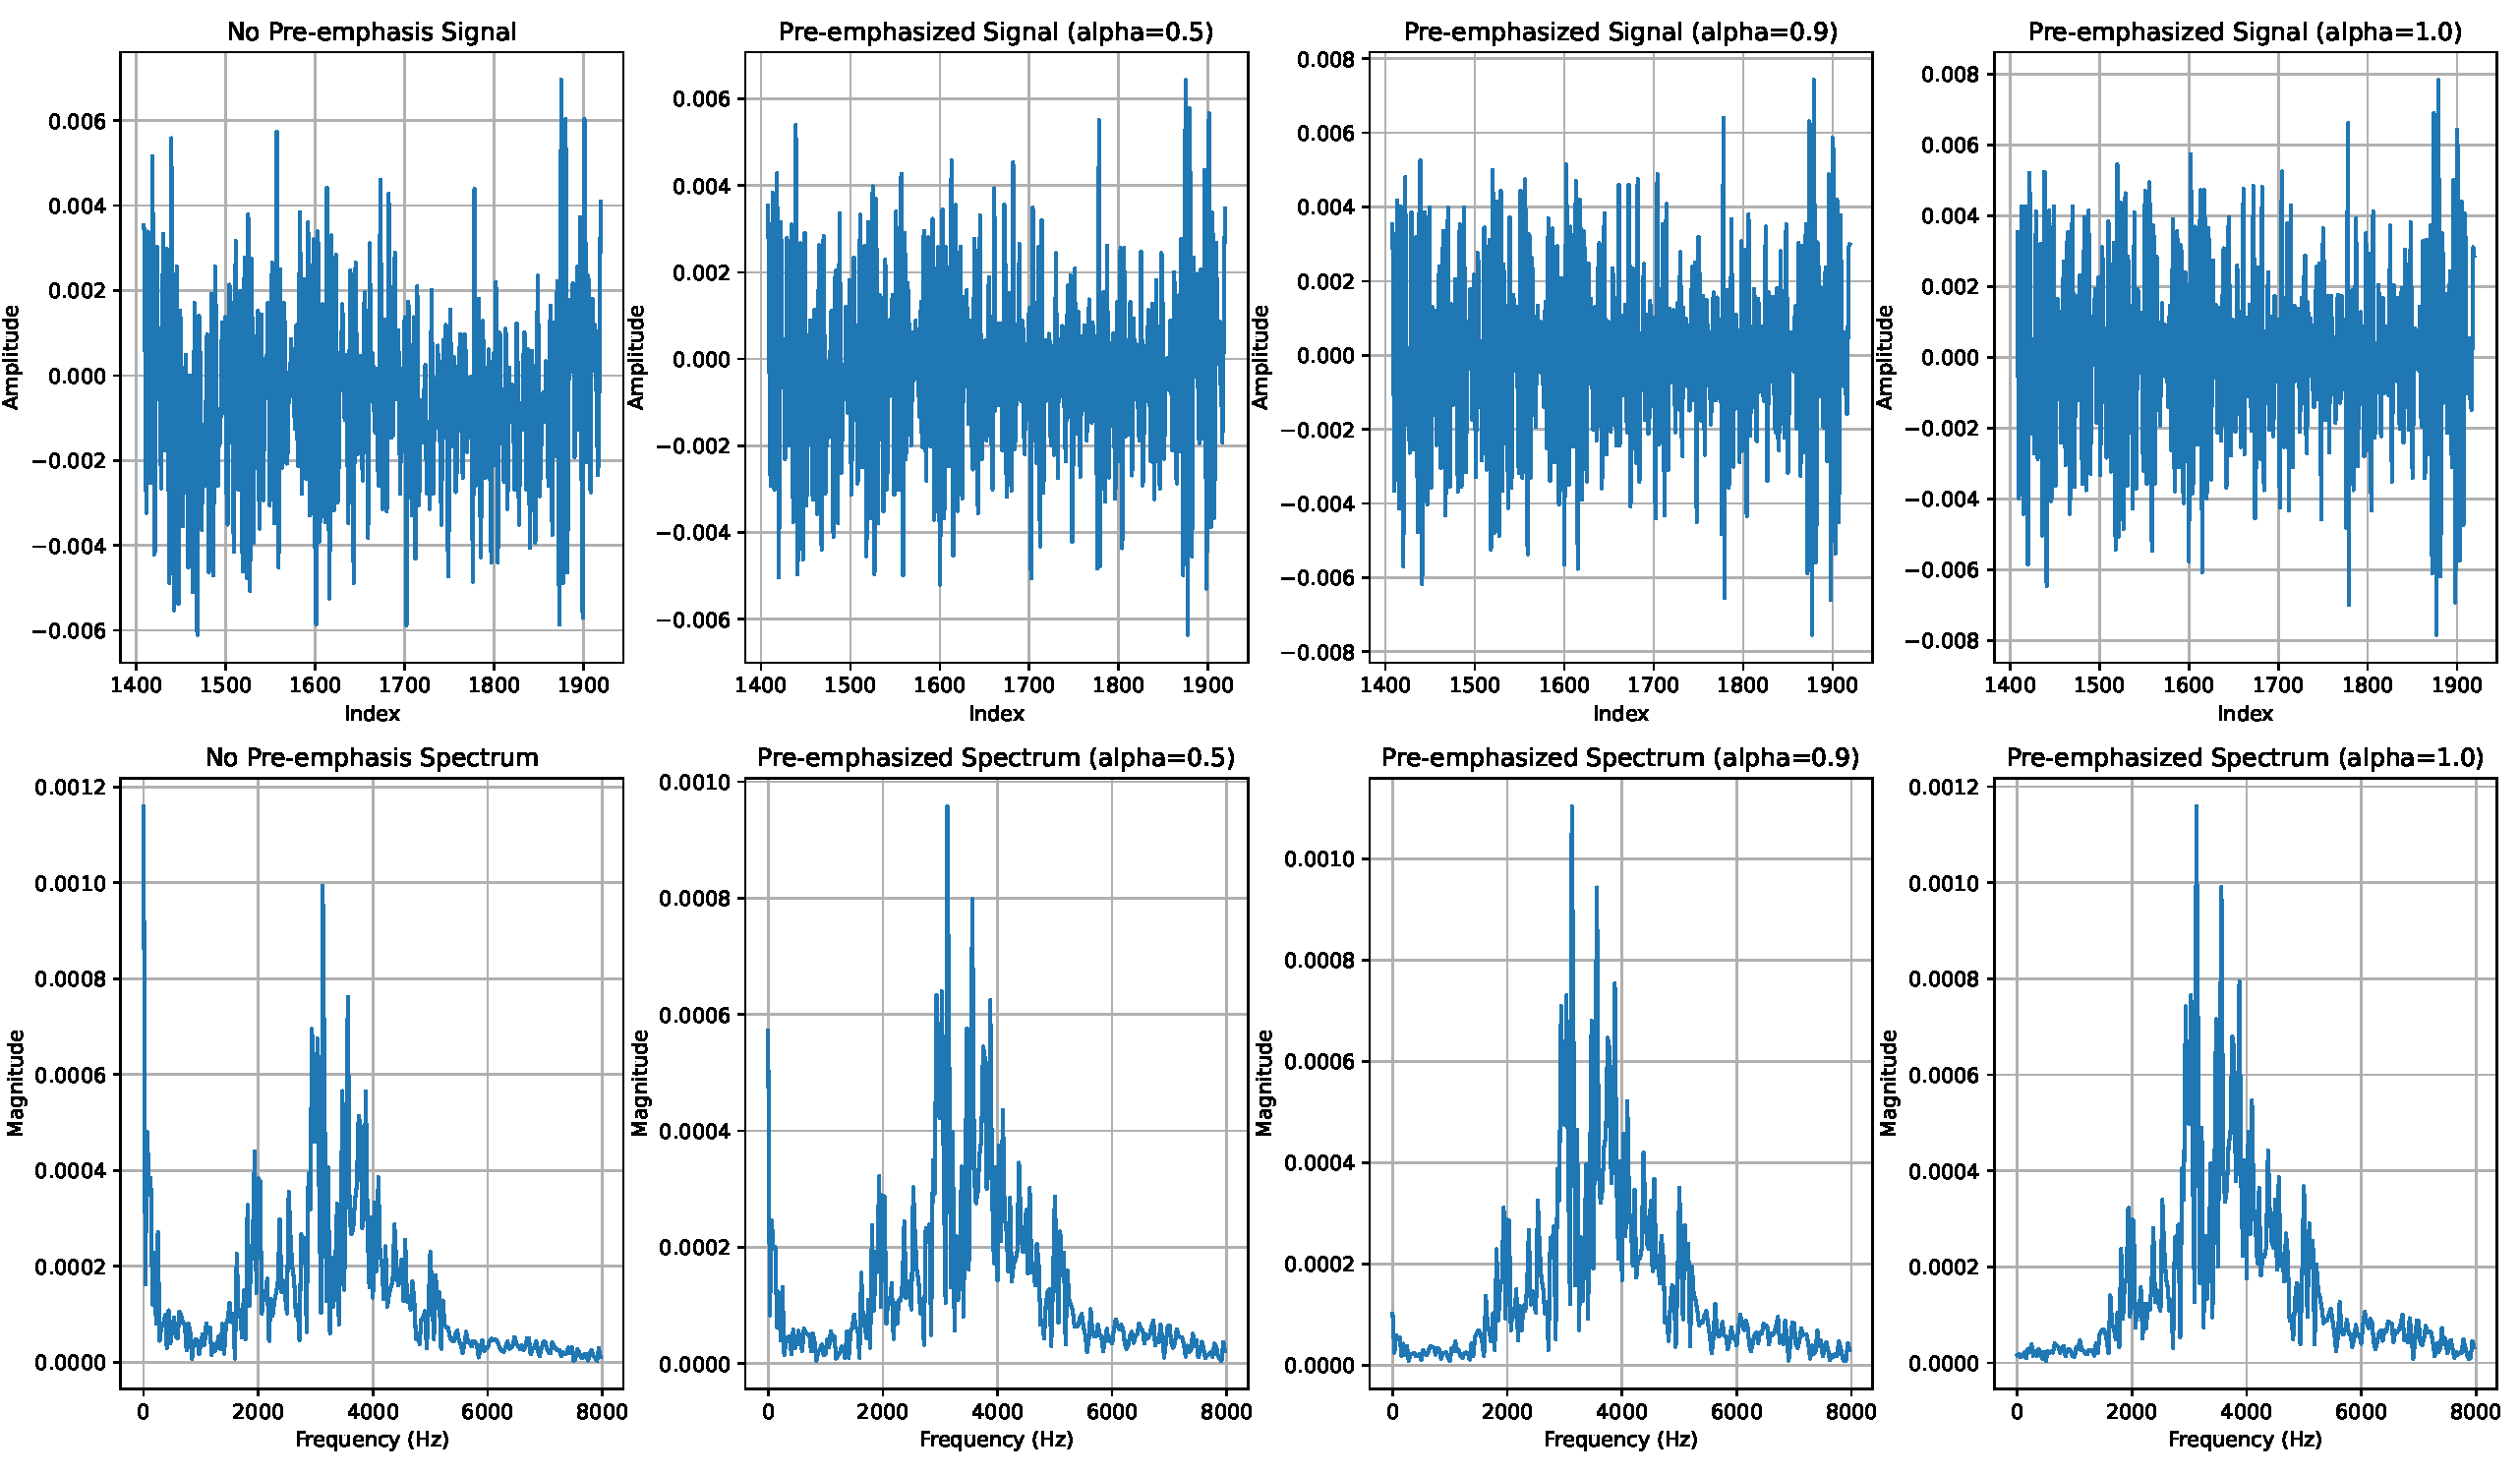
\includegraphics[width=0.5\textwidth]{figs/counting_on_pre_emphasis.pdf}
      \caption{预加重效果对比}
      \label{fig:counting_on_pre_emphasis}
    \end{figure}

    图\ref{fig:counting_on_pre_emphasis}中,可以看出,进行预加重处理之后,
    低频段的幅值会有明显的衰减,高频段的幅值有一定的增加,并且这种效果会随着$\alpha$的增大而加强。

    在本次作业中,我将始终保持对语音信号进行预加重处理,并选择$\alpha$为$0.97$。
  }
\end{enumerate}

\subsubsection{分帧}

\begin{enumerate}
  \item 
  {
    目的:
    \begin{itemize}
      \item 处理时变性:

      语音信号是时变的,即信号的特征在时间上是变化的
      (例如音高、音色、语速等)。然而,许多语音分析技术(如频谱分析、MFCC提取等)
      假设信号在短时间内是平稳的,即其统计特性不会随时间剧烈变化。通过分帧处理,
      我们可以将语音信号切割成较短的时间段(如$20ms$到$40ms$),并假设在这些短时间窗口内,
      信号的特性是相对稳定的
      \item 便于处理与分析:
  
      分帧处理使得信号变得更容易进行后续的特征提取(如MFCC、能量、零交叉率等)
      和模型训练(如语音识别模型)。通过将信号分成较小的帧,可以更精确地提取局部的频域特征和时域特征
      \item 提高分析精度:
  
      将信号分为小的帧后,每一帧的信号可以认为是近似平稳的,
      这使得在每一帧上进行傅里叶变换、功率谱分析等操作更为有效,可以更精确地捕捉到信号的局部特征
    \end{itemize}
  }
  \item
  {
    具体步骤:
    \begin{enumerate}
      \item 选择帧长和帧移:

      帧长指的是每一帧中的数据点数量,帧移指的是相邻两帧间隔的数据点数量。
      一般来说,帧长选择为$512$点到$4096$点,帧移选择为$128$点到$2048$点。
      本次实验中,采样率均为$16kHz$,对应时间长度为$32ms$到$256ms$,时间重叠为$8ms$到$128ms$。
      这是我们本次实验中一对重要的参数,具体对比实验详见\ref{tab:Linear SVM}及\ref{tab:Logistic Regression}
      \item 计算帧数与补零:
  
      设信号的总长度为$N$,帧长为$L$,帧移为$S$,帧数$n_{frames}$有以下两种计算方式:
      \begin{itemize}
        \item 下取整,对应忽略信号末尾多余的数据点,并不进行补零操作:
        \begin{equation}
          n_{frames} = \lfloor \frac{N - L}{S} \rfloor + 1
          \label{eq:floor}
        \end{equation}
        \item 上取整,对应不忽略信号末尾数量小于帧长的数据点,并进行补零操作:
        \begin{equation}
          n_{frames} = \lceil \frac{N - L}{S} \rceil + 1
          \label{eq:ceil}
        \end{equation}
        对应的补零数量$n_{paddle}$为:
        \begin{equation}
          (n_{frames} - 1) * S + L - N
        \end{equation}
      \end{itemize}
      \item 滑动窗口:

      在分帧过程中,每一帧的信号由一个滑动窗口提取,窗口的起始位置由帧移决定。
      具体地,每一帧的信号从上一个帧的起始位置向前滑动帧移的距离。
      第$i$帧$x_i$可以通过以下公式获得:
      \begin{equation}
        x_i = x\left[i\cdot S, i\cdot S + L \right]
        \label{eq:enframe}
      \end{equation}
      其中$x$为经过补零(下取整不需要补零)后的语音信号
      
    \end{enumerate}
  }
  \item
  {
    伪代码:
    \begin{algorithm}
      \caption{分帧处理伪代码}
      \label{alg:enframe}
      \begin{algorithmic}[1]
      \State \textbf{Input:} $x$, $L$, $S$, $ceil\_or\_floor$
      \If{$ceil\_or\_floor = 'ceil'$}
          \State $n\_frames \gets \left\lceil \frac{\text{len}(x) - L}{S} \right\rceil + 1$
      \ElsIf{$ceil\_or\_floor = 'floor'$}
          \State $n\_frames \gets \left\lfloor \frac{\text{len}(x) - L}{S} \right\rfloor + 1$
      \EndIf
      \State $x\_framed \gets \text{Zeros}((n\_frames, L))$
      \State $padlen \gets (n\_frames - 1) \times S + L$
      \State $zeros \gets \text{Zeros}((\max(0 ,padlen - \text{len}(x)),))$
      \State $padsignal \gets x \cup zeros$
      \For{$i = 0 \rightarrow n\_frames - 1$}
          \State $x\_framed[i] \gets padsignal[i \times S : i \times S + L]$
      \EndFor
      \State \textbf{Output:} $x\_framed$
      \end{algorithmic}
    \end{algorithm}

    \begin{enumerate}
      \item 传入参数:一维语音信号$x$,帧长 $L$,帧移$S$,以及选择上取整或下取整的标志
      \item 计算帧数
      \item 初始化分帧矩阵
      \item 计算补零后的总长度
      \item 将补零后的信号连接到原信号后面
      \item 最后返回分帧后的信号矩阵
    \end{enumerate}
  }
\end{enumerate}

\subsubsection{加窗}
\begin{enumerate}
  \item 
  {
    目的:
    \begin{itemize}
      \item 减少边界效应:

      语音信号通常是连续的,但在实际处理中,我们是将其划分为一个个短时帧,每一帧都是有限长度的。
      直接截断信号的每一帧会产生突然的边界,这种边界会引入高频噪声,影响信号的频谱特性。
      加窗的操作通过平滑帧的边界,减少这种不自然的突变,减小频谱泄漏
      \item 提高频谱分析的准确性:

      通过对每一帧信号进行加窗处理,可以使得每一帧信号在时域上更加平滑,
      这样进行傅里叶变换时能获得更加准确的频谱,特别是在低频部分的分辨率和信号的可辨识度上有显著改善
      \item 改善信号的平稳性:

      语音信号往往在时间上是非平稳的,短时分析需要假设信号在每一小段时间内是平稳的。
      加窗操作帮助保证每一小段时间内的信号变化较小,从而更符合短时平稳的假设,便于进一步进行频谱分析
    \end{itemize}
  }
  \item 
  {
    典型窗函数:
    \begin{itemize}
      \item \textbf{矩形窗:}
      \begin{equation}
        w(n) = 
        \begin{cases} 
        1, & 0 < n < N-1 \\
        0, & \text{其他}
        \end{cases}
        \label{eq:retangle}
      \end{equation}

      \item \textbf{汉明窗(Hamming):}
      \begin{equation}
        w(n) = 
        \begin{cases} 
        0.54 - 0.46 \cos\left( \frac{2\pi n}{N-1} \right), & 0 < n < N-1 \\
        0, & \text{其他}
        \end{cases}
        \label{eq:Hamming}
      \end{equation}

      \item \textbf{汉宁窗 (Hann):}
      \begin{equation}
        w(n) = \frac{1}{2} \left[ 1 - \cos\left( \frac{2\pi n}{N-1} \right) \right], \quad 0 < n < N-1
        \label{eq:Hann}
      \end{equation}
  
      \item \textbf{巴特利特窗 (Bartlett) (三角形窗):}
      \begin{equation}
        w(n) = 
        \begin{cases} 
        \dfrac{2n}{N-1}, & 0 < n < \dfrac{N-1}{2} \\
        2 - \dfrac{2n}{N-1}, & \dfrac{N-1}{2} < n < N-1 
        \end{cases}
        \label{eq:Bartlett}
      \end{equation}

      \item \textbf{布莱克曼窗 (Blackman):}
      \begin{equation}
        \begin{split}
          w(n) = 0.42 - 0.5 \cos\left( \frac{2\pi n}{N-1} \right)\\
           + 0.08 \cos\left( \frac{4\pi n}{N-1} \right), \quad 0 < n < N-1
        \end{split}
      \end{equation}

  \end{itemize}
  }
  \item 
  {
    不同窗函数以及窗长直观对比:
    \begin{figure*}[h]
      \centering
      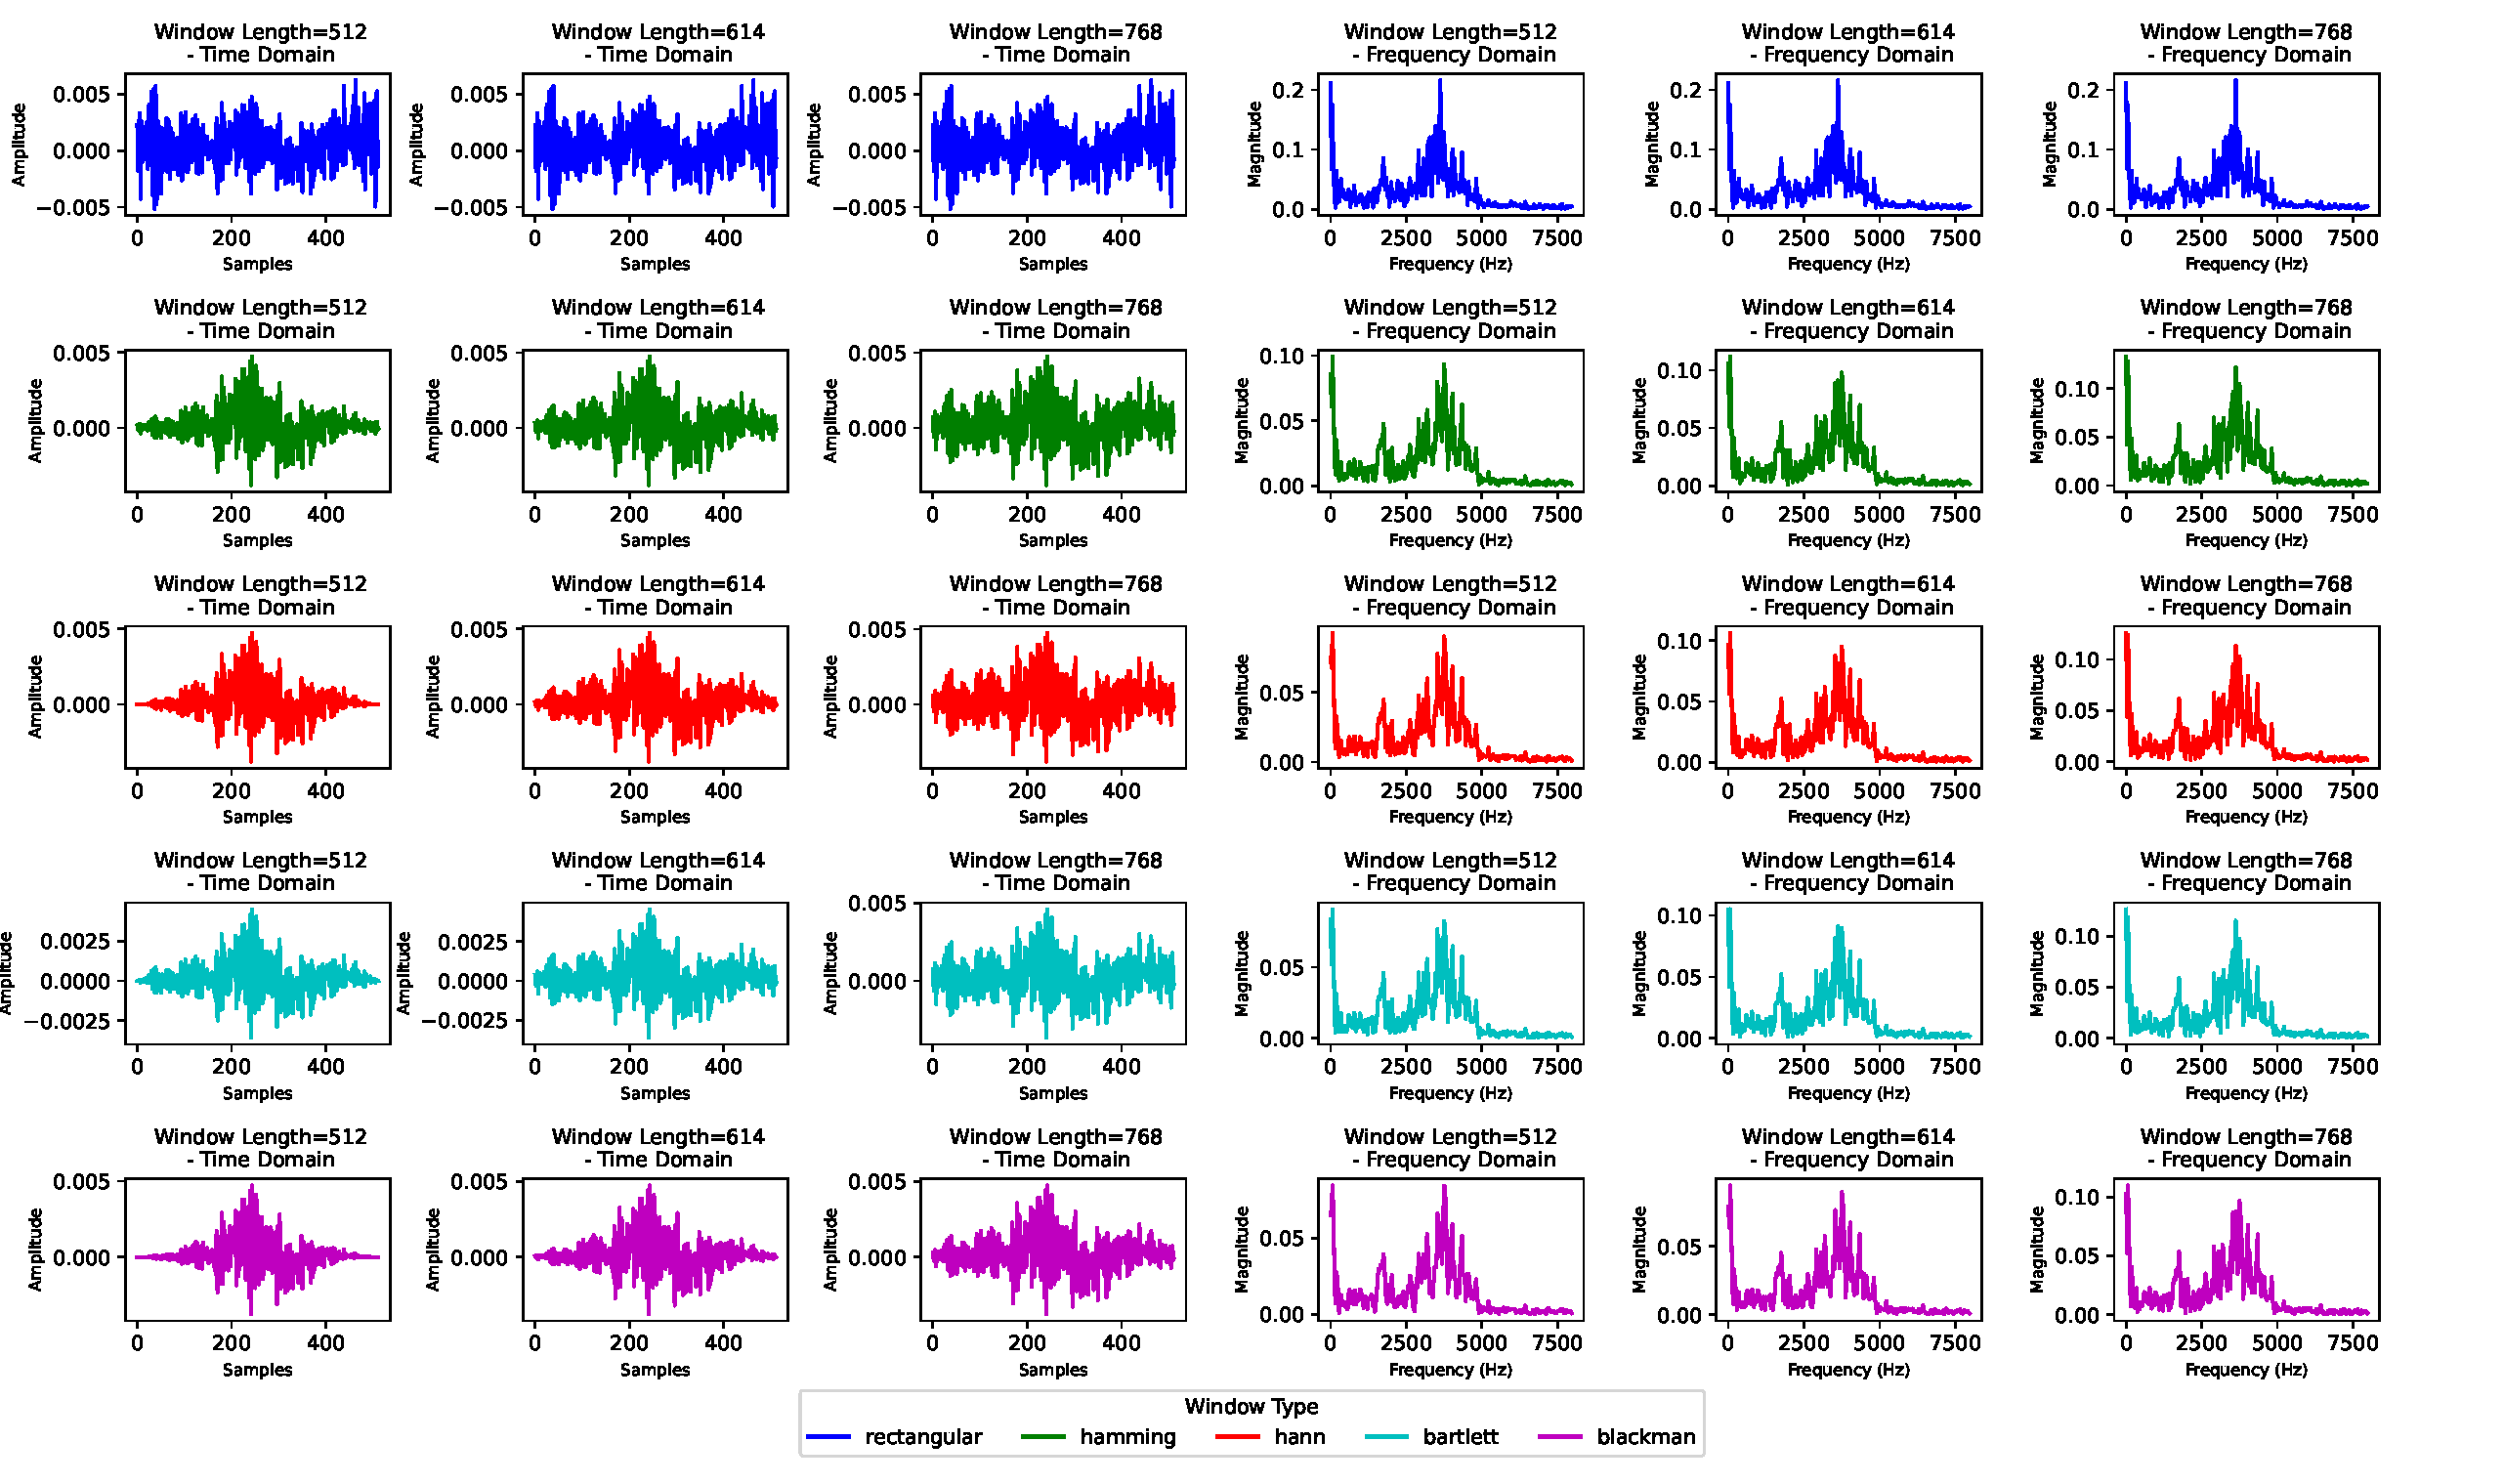
\includegraphics[width=\textwidth]{figs/counting_on_windows.pdf}
      \caption{不同窗窗函数以及窗长作用效果对比}
      \label{fig:counting_on_windows}
    \end{figure*}

    我取出了开发集中的一段语音信号,截取了帧长为$512$的一帧信号,
    并使用上述五种窗函数,得到信号的时域的波形图以及频域的谱图(图\ref{fig:counting_on_windows})。
    其中,我选用了$3$种不同的窗长(为保证信号的完整性,窗长大于帧长,并居中对齐):
    \begin{itemize}
      \item 等于帧长$(512)$
      \item 帧长的$1.2$倍$(614)$
      \item 帧长的$1.5$倍$(768)$
    \end{itemize}
    评价一个窗函数的性能的指标主要有:
    \begin{itemize}
      \item 主瓣宽度
      \item 旁瓣抑制
      \item 频谱泄露
      \item 实现效率
    \end{itemize}
    综合上述指标,我选取了\textbf{汉宁窗}(\ref{eq:Hann}),并设置窗长与帧长一致,
    这样设置在保证主瓣宽度的前提下,能有较好的旁瓣抑制,并且计算复杂度也较低。
  }
\end{enumerate}


\subsubsection{短时能量}
\begin{enumerate}
  \item 
  {
    原始描述:

    一帧内的采样点的平方和
  }
  \item 
  {
    给人耳听觉的直观感受:
    \begin{itemize}
      \item 较高的短时能量通常意味着声音较大或较响亮,这对应着人耳感知的音量增强
      \item 较低的短时能量意味着信号较弱或较安静,这在人耳中会感觉到声音减弱或不明显
    \end{itemize}
  }
  \item
  {
    计算公式:
    \begin{equation}
      E = \sum_{i=0}^{N-1}s_i^2
      \label{eq:energies}
    \end{equation}
    其中,$s_i$为语音帧$s$中的第$i$个采样点
  }
  \item
  {
    可视化:

    我取出了开发集中的一段语音信号,进行帧长和帧移分别为$512, 128$的分帧,分别求取每一帧能量,
    并取出第$100$帧对应的波形图和能量,得到图\ref{fig:energies}
    \begin{figure}
      \centering
      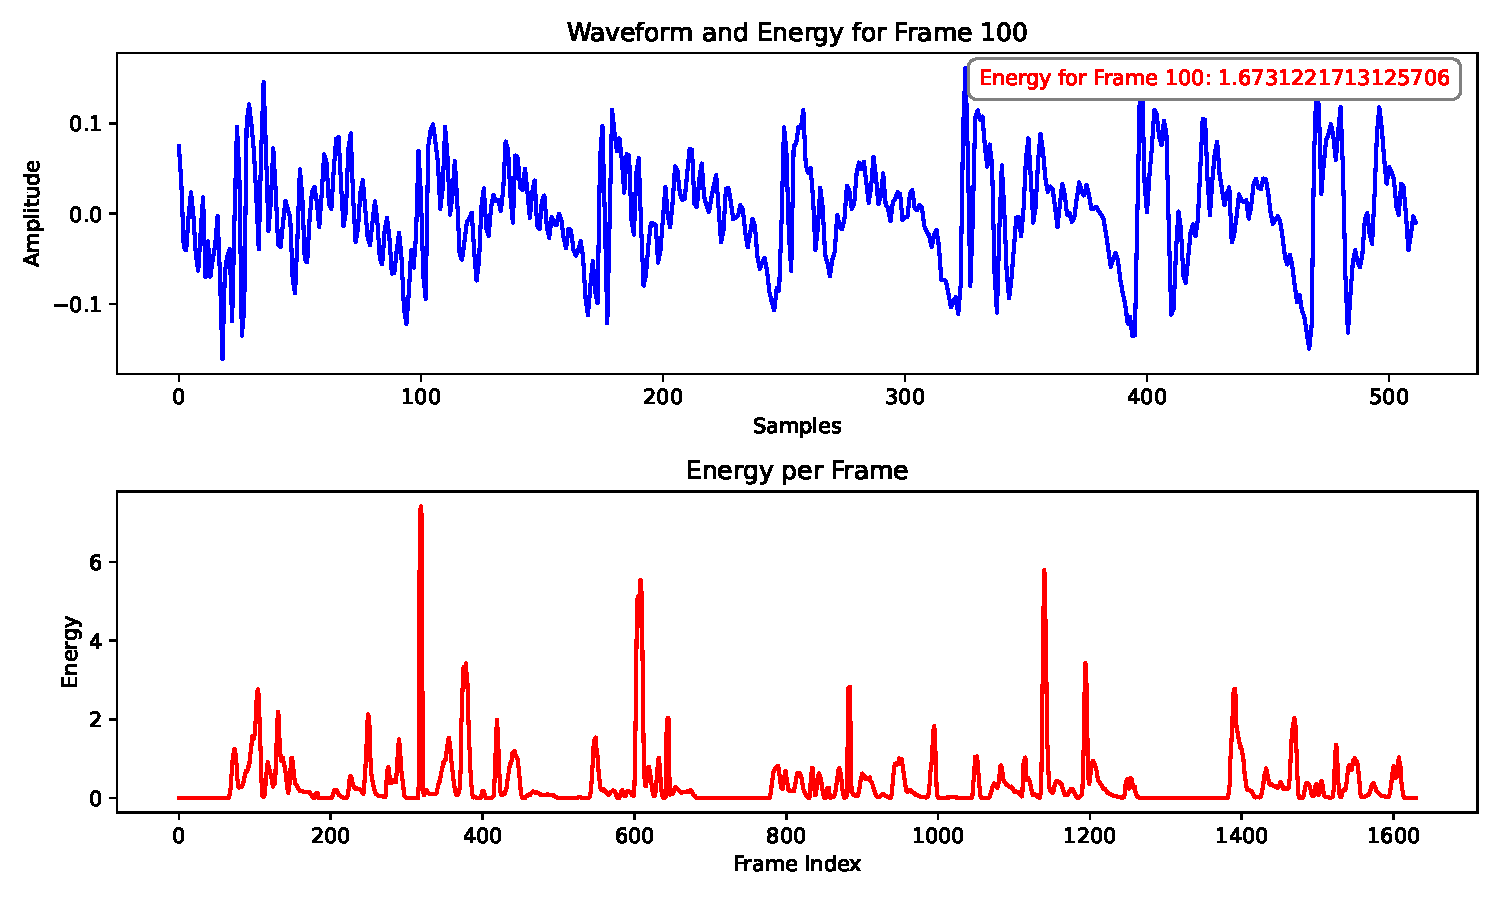
\includegraphics[width=0.5\textwidth]{figs/energies.pdf}
      \caption{短时能量}
      \label{fig:energies}
    \end{figure}
  }
\end{enumerate}

\subsubsection{短时过零率}
\begin{enumerate}
  \item 
  {
    原始描述:

    每一帧中采样点正负反复的次数(跨越零点的次数)。
    清音的过零率较大,浊音的过零率较小。
  }
  \item 
  {
    给人耳听觉的直观感受:
    \begin{itemize}
      \item 短时过零率通常与信号的音高和音调变化有关。高过零率的信号通常意味着信号有快速的变化,可能对应着清脆、高频的声音,比如某些辅音或短促的音

      \item 低过零率的信号则意味着信号变化较慢,通常代表的是低频的声音,或者是语音中的元音部分
      
      \item 高过零率在语音的快速、急促或高音调部分较为常见,而低过零率常见于语音的平稳、低音调部分
    \end{itemize}
  }
  \item 
  {
    计算公式:
    \begin{equation}
      Z = \frac{1}{2}\sum_{i=0}^{N-1}\mid sgn(s_i) - sgn(s_{i-1})\mid
      \label{eq:ZRC}
    \end{equation}

    其中,
    \begin{equation}
      sgn(x) 
      \begin{cases} 
      1, &x \geqslant 0 \\
      0, &x < 0  
      \end{cases}
      \label{eq:Sign}
    \end{equation}
  }
  \item 
  {
    可视化:

    我取出了开发集中的一段语音信号,进行帧长和帧移分别为$512, 128$的分帧,分别求取每一帧过零率,
    并取出第$100$帧对应的波形图和过零率,得到图\ref{fig:ZCR}
    \begin{figure}
      \centering
      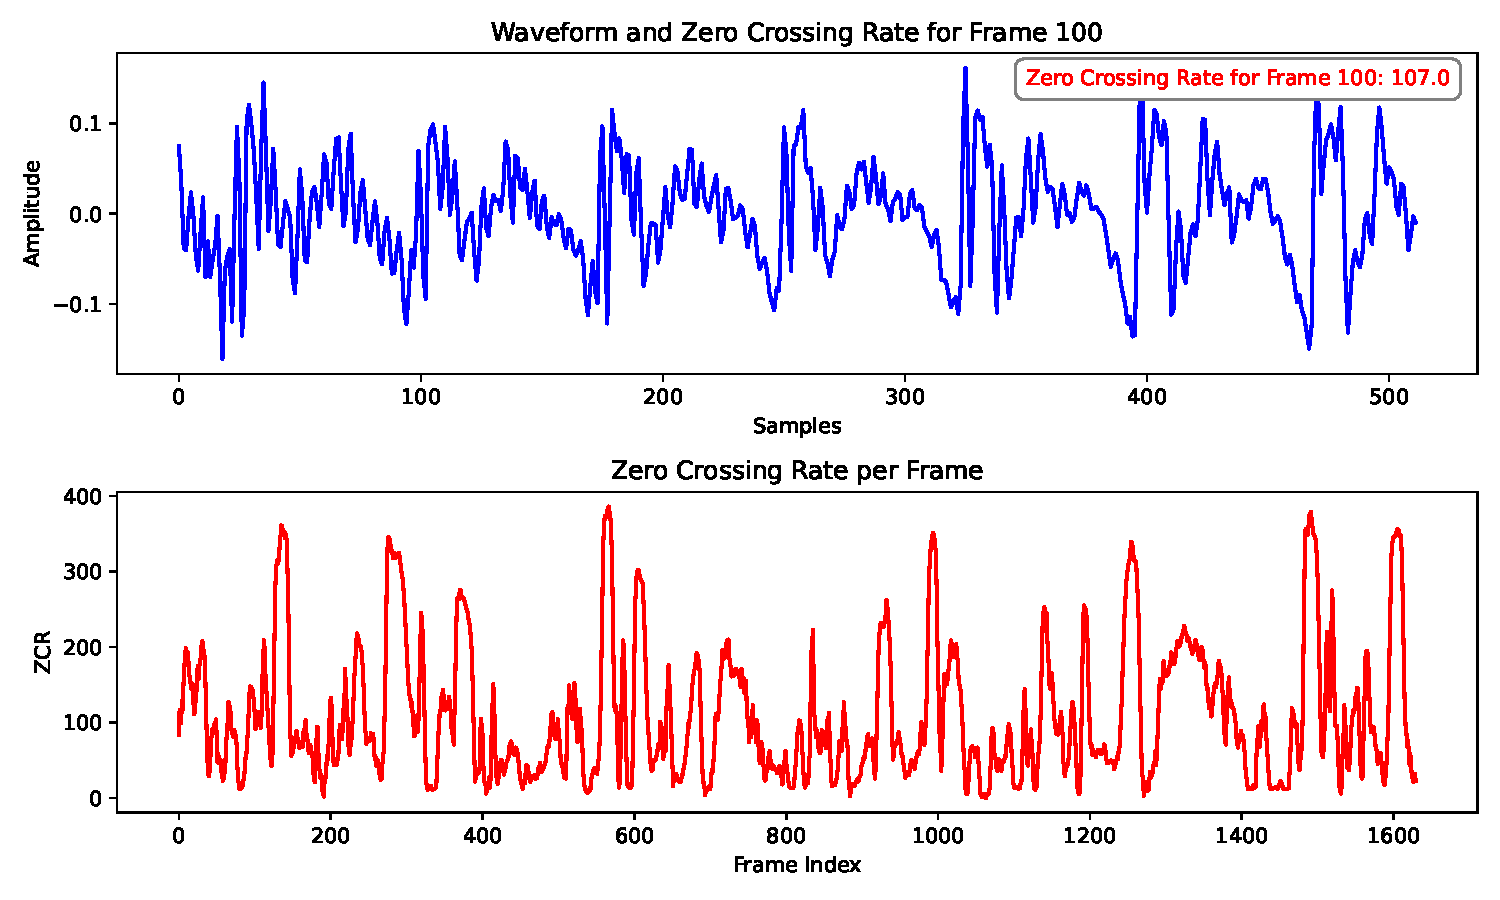
\includegraphics[width=0.5\textwidth]{figs/ZCR.pdf}
      \caption{短时过零率}
      \label{fig:ZCR}
    \end{figure}
  }
\end{enumerate}

\subsubsection{短时基频}
\begin{enumerate}
  \item 
  {
    描述:

    基频(Pitch)或者基本频率(Fundamental Frequency)$F_0$是人类语音的最低的频率,它是组成语音中更高频率成分的基础。
    \begin{itemize}
      \item 浊音部分有明显的周期性,而清音部分仅仅是随机振动
      \item 人类的$F_0$范围大概是$60Hz$到$300Hz$
    \end{itemize}
  }
  \item 
  {
    给人耳听觉的直观感受:
    \begin{itemize}
      \item 基频与人耳的音高感知密切相关。较高的基频通常给人以尖细、高亢的声音感受(例如女性或儿童的语音),而较低的基频则给人以低沉、粗哑的声音感受(例如男性或低沉的音调)

      \item 基频的变化往往与语音的情感、语气、语调相关。例如,语音中的上扬或下滑基频往往用来表示疑问、惊讶或情绪波动
      
      \item 基频对于语音音调和声学韵律的表达至关重要,能够影响听者对说话者的性别、年龄及情感的判断
    \end{itemize}
  }
  \item 
  {
    原理:

    我使用的是最简单的\textbf{自相关法},自相关系数的定义如下:
    \begin{equation}
      R(l) = \sum_{i=0}^{N-l-1}s_{i+l}\cdot s_{i}
    \end{equation}
    当$l=nT_0$($T_0$为基音周期), $n = 1, 2, \dots$时,$R(l)$函数接近局部最大值。

    这个算法涉及到自相关系数的求取,这能用\emph{numpy.correlate}快捷地实现,这也是我选择自相关法的主要原因。
  }
  \item 
  {
    基频提取:
    \begin{enumerate}
      \item 计算自相关函数的值$R(l)$
      \item 设定$T_{min}$和$T_{max}$,限定基音周期$T$的范围
      \item 在$0.5\cdot T_{min} < l < 1.5\cdot T_{max}$的范围内搜索得到基音$\hat{T_0}$对应序号$\hat{l_0}$
      \item 由基频$F_0$,基音周期$T$和采样率$f_s$之间的关系\ref{eq:fs_equality}得到基频$\hat{F_0}$
      \begin{equation}
        F_0 = \frac{1}{T_0} = \frac{f_s}{l_0}
        \label{eq:fs_equality}
      \end{equation}
    \end{enumerate}
  }
  \item 
  {
    代码实现:
    \begin{lstlisting}[language=python]
# 基频提取
def pitch_detection(frame, t_min: float = 0.003, t_max:float = 0.01):
  # 计算自相关
  corr = np.correlate(frame, frame, mode='same')
  # 找到第一个峰值的位置
  peak_index = np.argmax(corr[int(0.5 * t_min * fs) : int(1.5 * t_max * fs)]) + int(0.5 * t_min * fs)
  # 计算基频
  pitch = fs / peak_index
  return pitch
    \end{lstlisting}
    \begin{enumerate}
      \item 传入参数:单独一帧语音信号,参数\emph{t\_min}和\emph{t\_max}
      \item 计算自相关
      \item 找到第一个峰值
      \item 计算并返回基频
    \end{enumerate}
  }
  \item 
  {
    参数设置:

    由于人类的$F_0$的范围大概是$60Hz$到$300Hz$,
    而由于本次实验中有背景噪声存在,为提高准确率,我将基频的最低值假定为$100Hz$,
    故设置$T_{min}$和$T_{max}$分别为:$0.01$和$0.003$(单位:$s$)。
  }
  \item 
  {
    平滑操作:

    基频提取的本质是从每帧的信号中获得周期性特征。

    基频提取通常会受到噪声和语音特征变化的影响,导致估计的基频出现不规则的波动。

    为了得到更加平稳的基频曲线,我们可以对基频进行平滑操作,去除这些波动。

    在本次实验中,我取出了开发集中的一段语音信号,以帧长和帧移分别为$(2048, 512)$和$(512, 128)$进行分帧,
    并对比了中值滤波\emph{Median Filter},卷积滤波\emph{Convolve Filter}和有限脉冲响应滤波其\emph{FIR},
    得到图\ref{fig:smooth1}和\ref{fig:smooth2}中的效果。
    \begin{figure}[h]
      \centering
      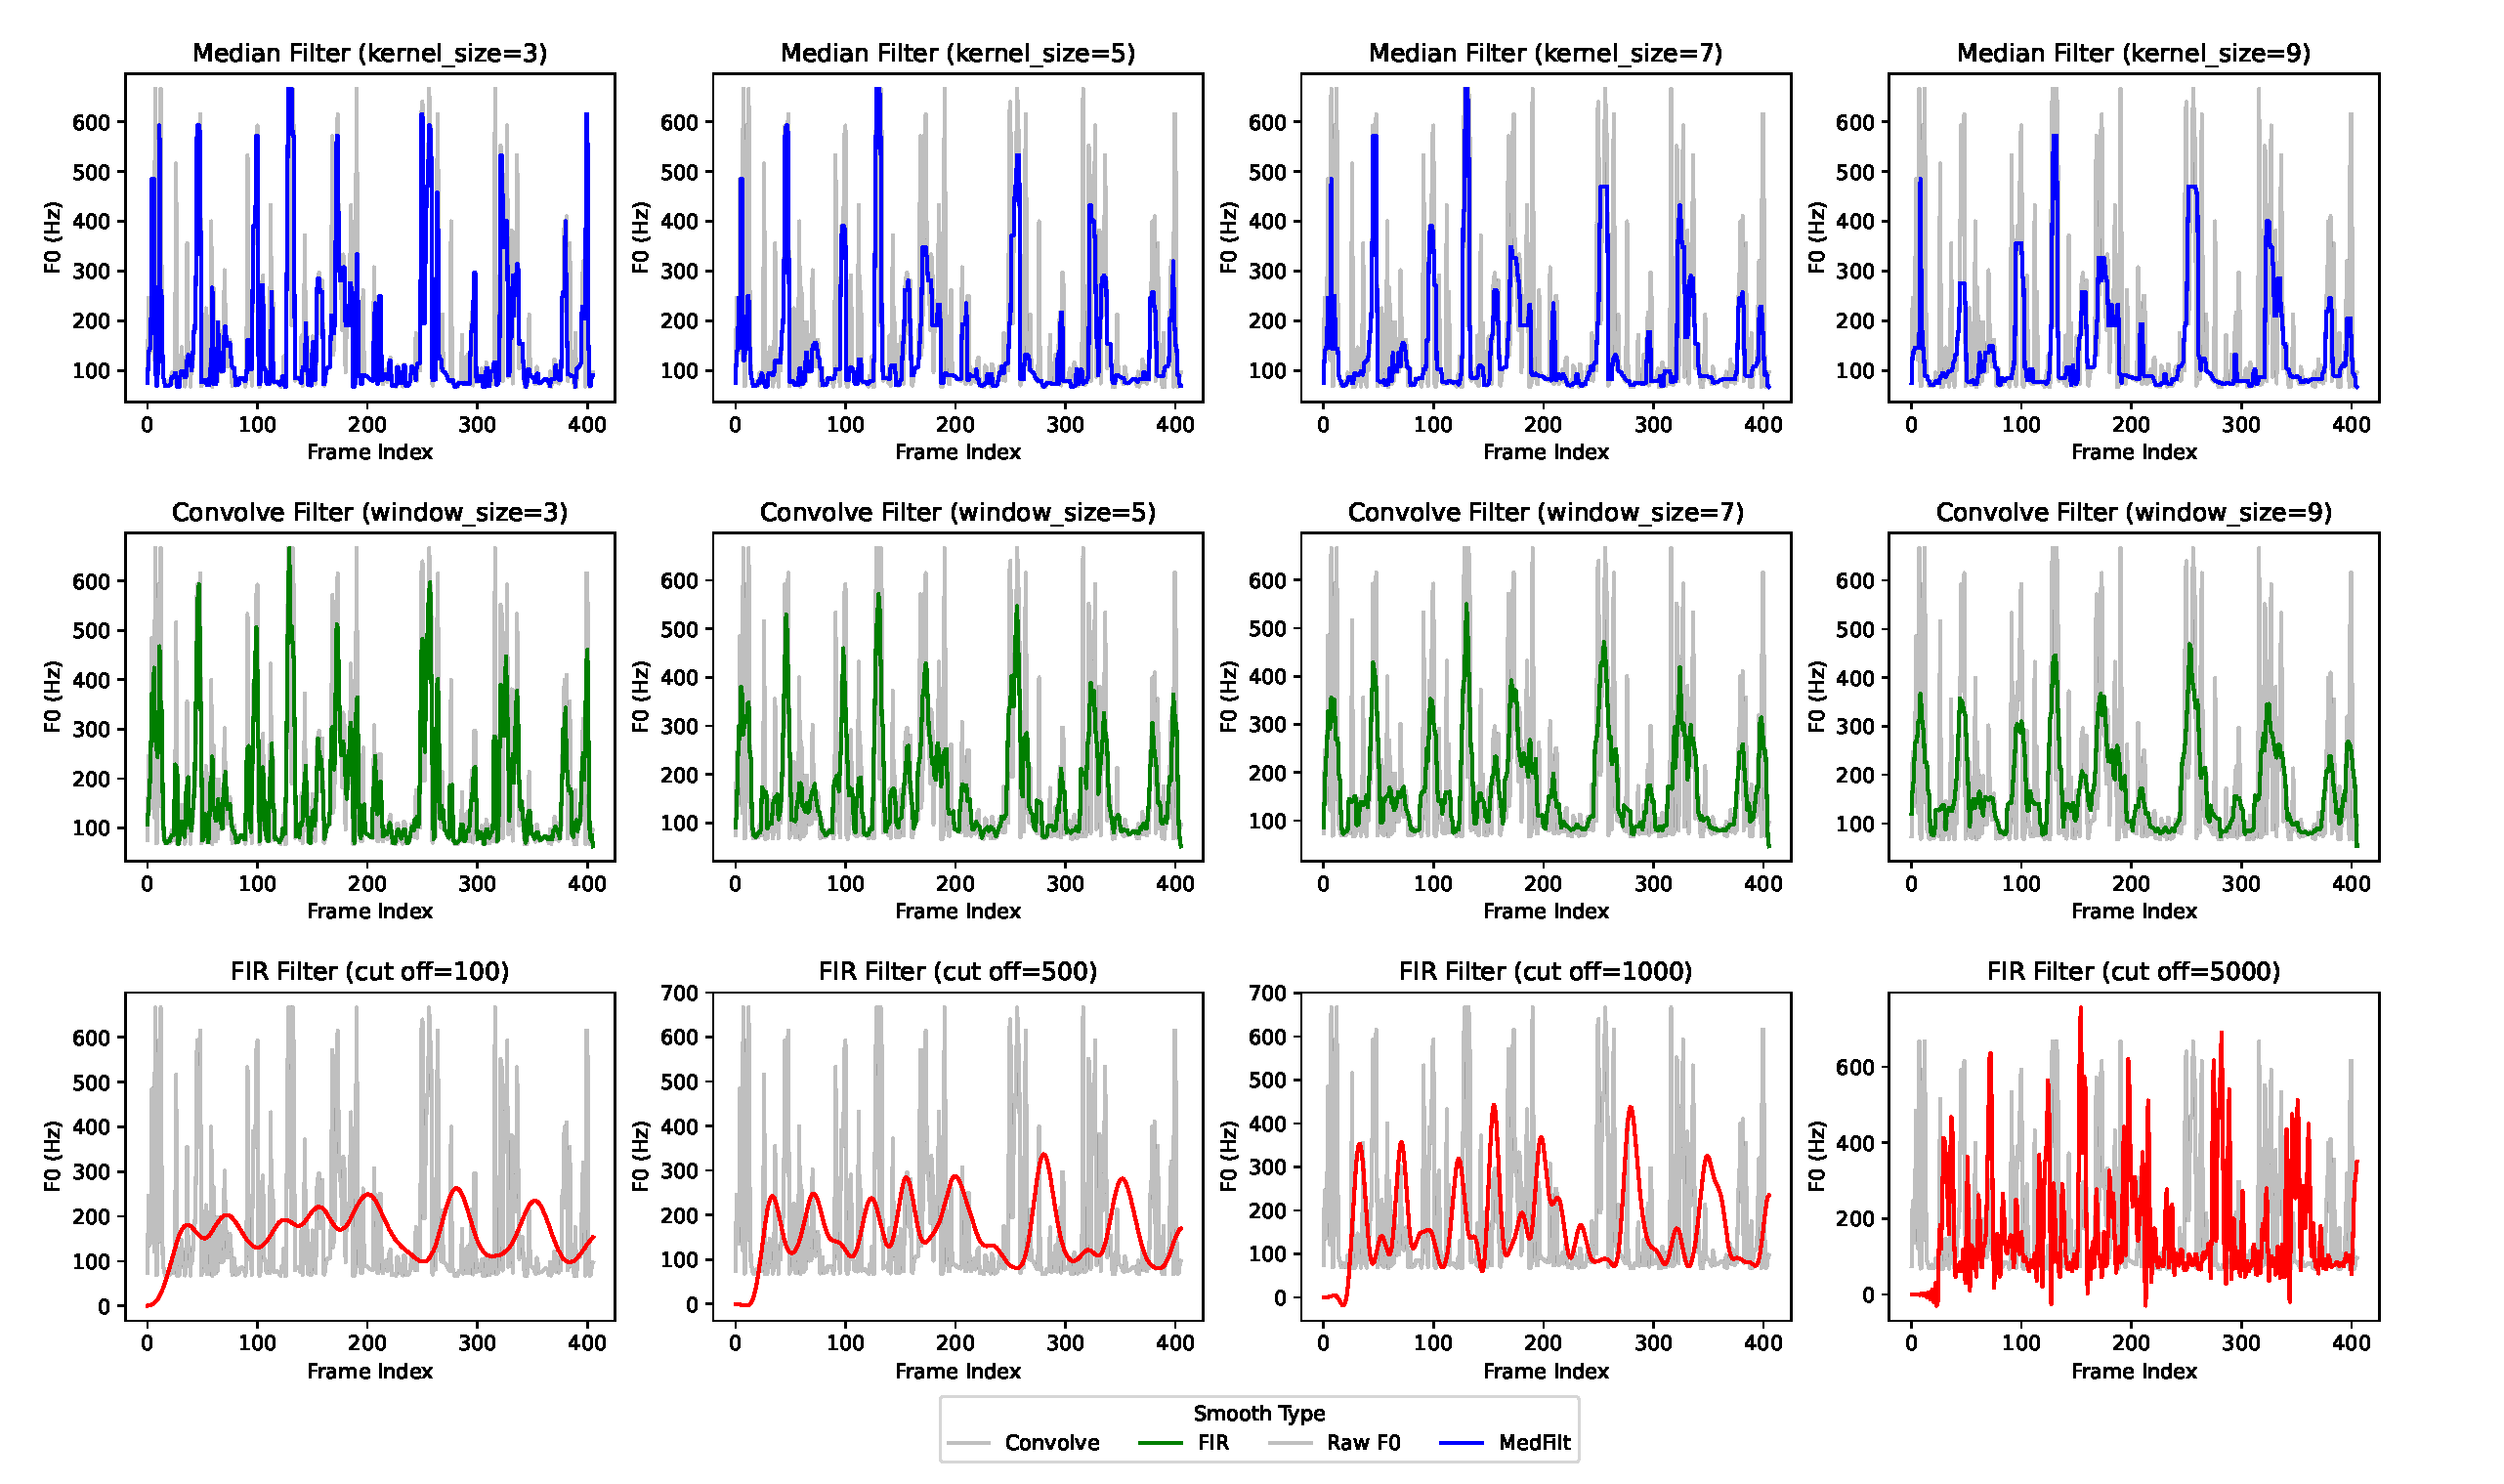
\includegraphics[width=0.5\textwidth]{figs/counting_on_smooth.pdf}
      \caption{不同平滑操作以及不同参数作用效果对比,对应帧长和帧移$(2048, 512)$}
      \label{fig:smooth1}
    \end{figure}

    \begin{figure}[H]
      \centering
      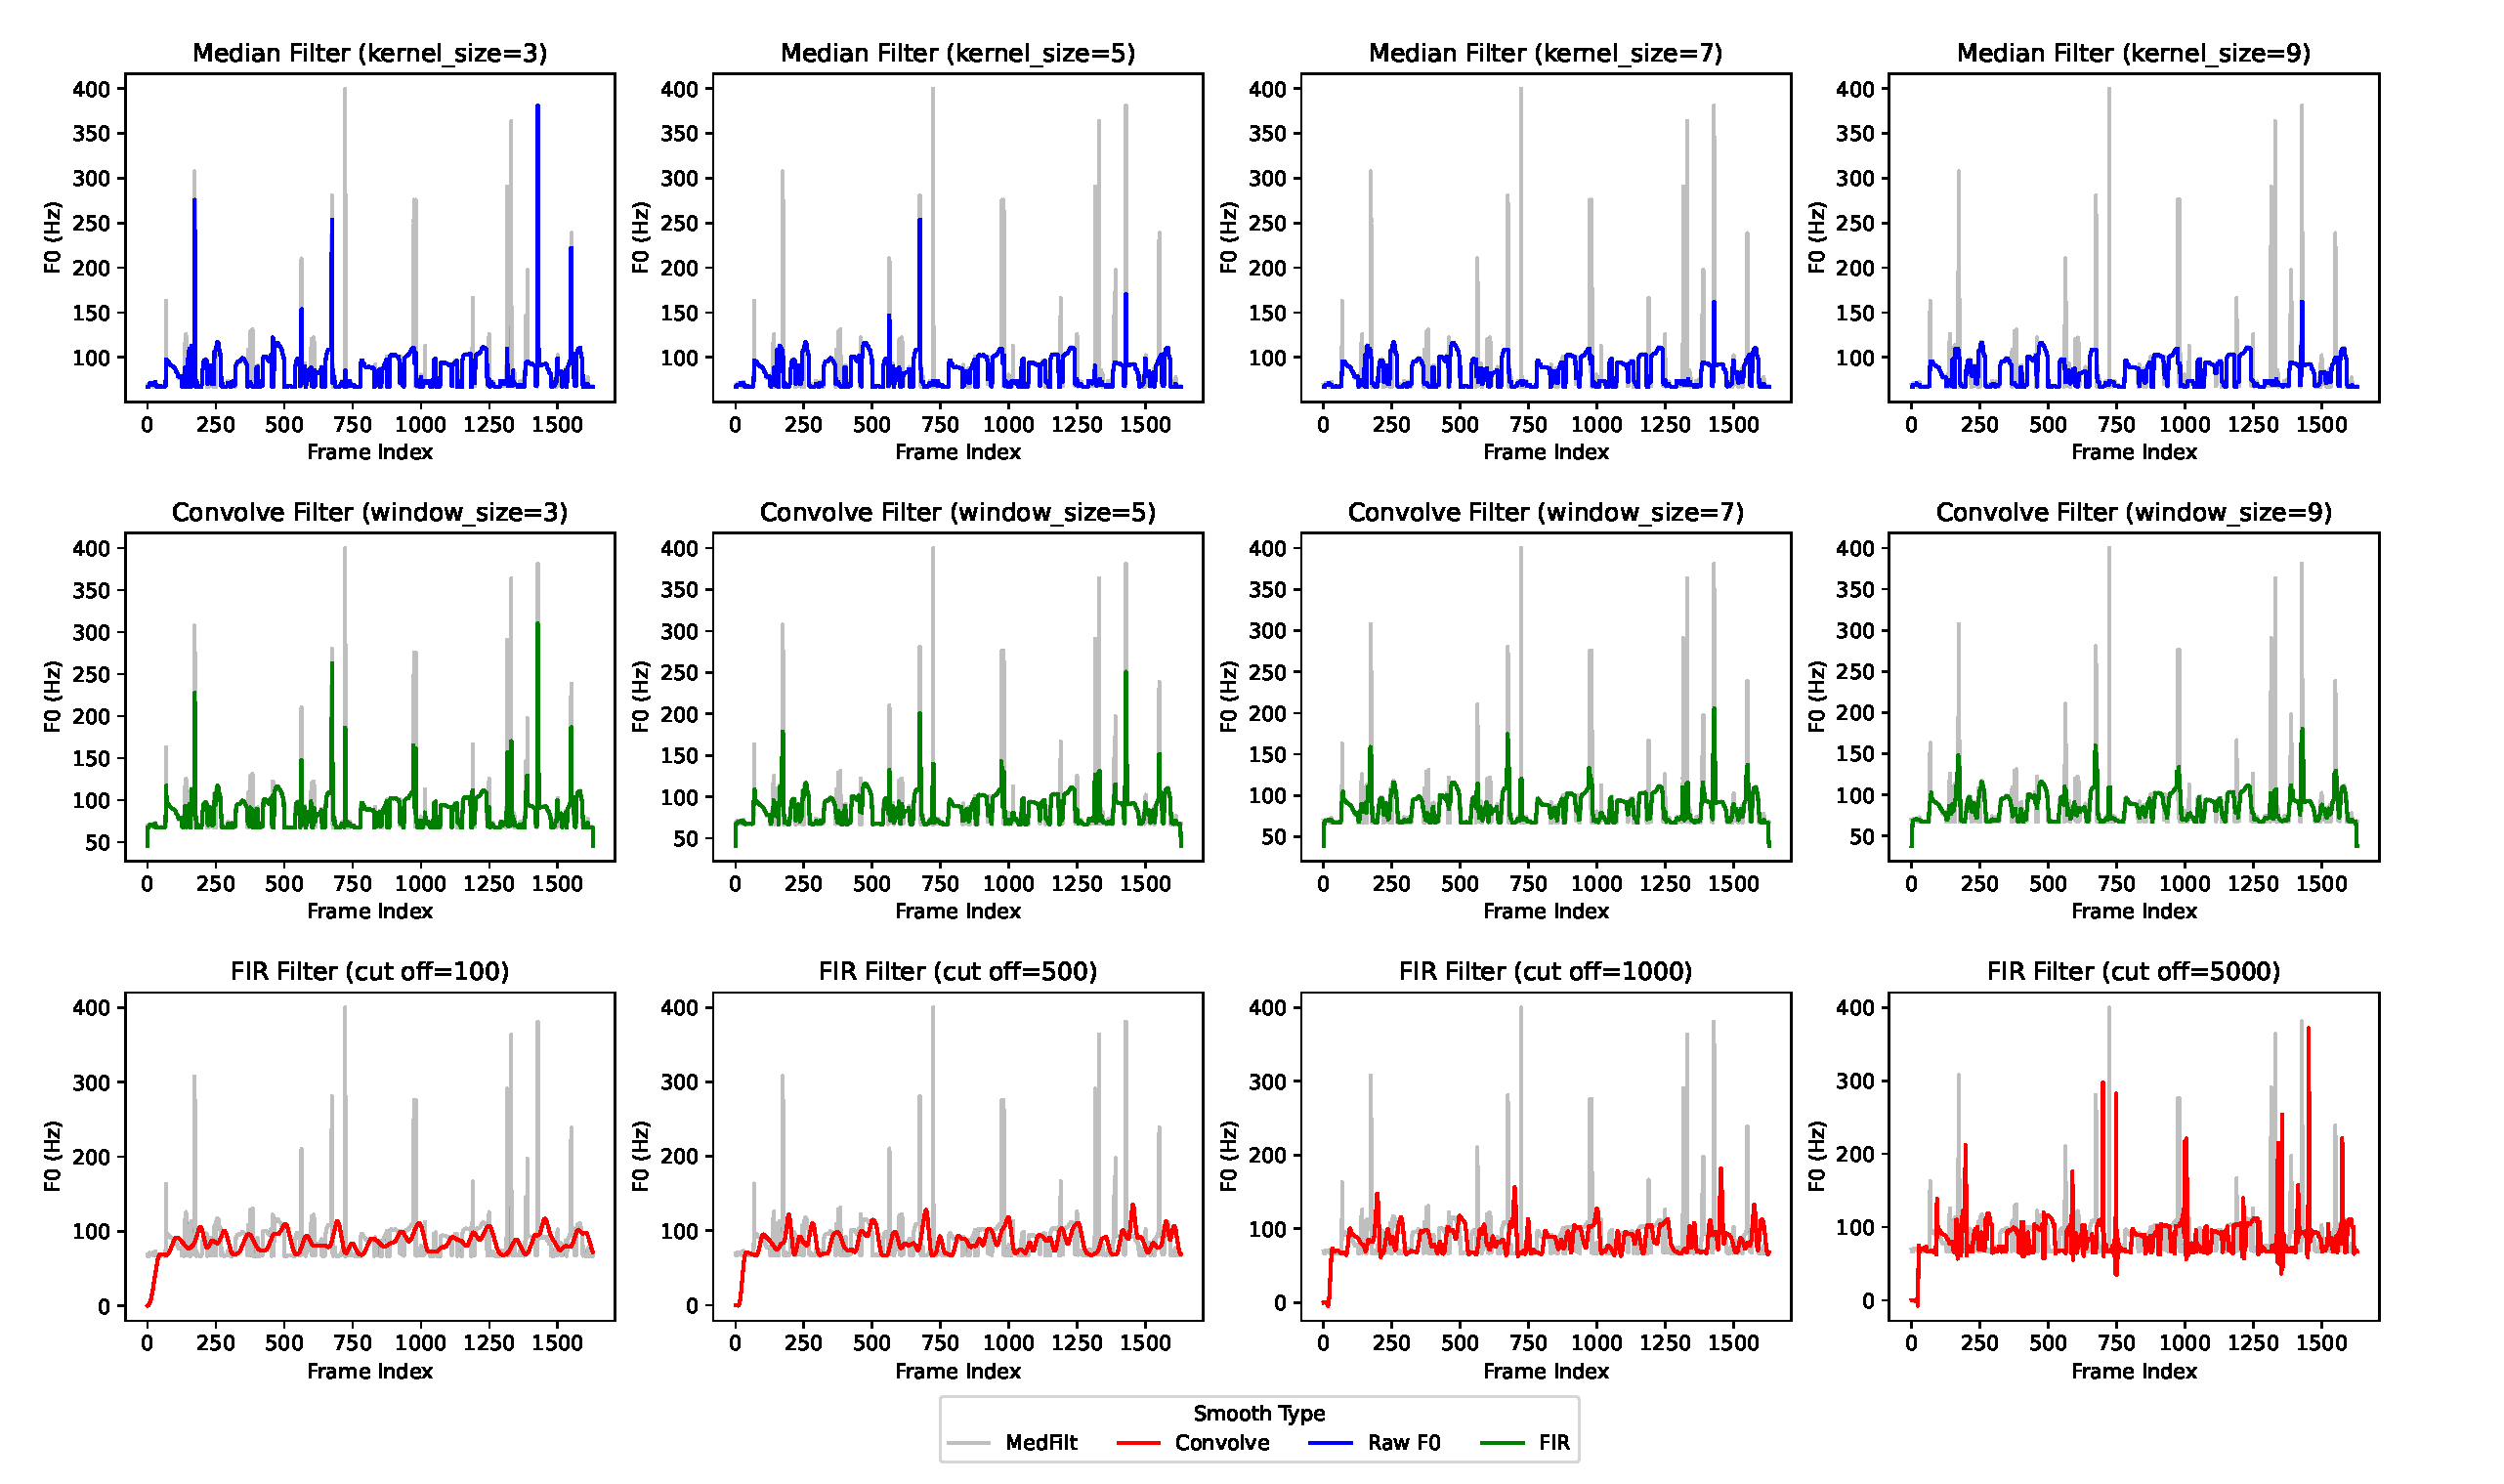
\includegraphics[width=0.5\textwidth]{figs/counting_on_smooth_2.pdf}
      \caption{不同平滑操作以及不同参数作用效果对比,对应帧长和帧移$(512, 128)$}
      \label{fig:smooth2}
    \end{figure}

    其中,卷积滤波中使用的滤波器核是均匀平均滤波器。

    在帧长帧移组合为$(2048, 512)$时(如图\ref{fig:smooth1}),中值滤波器可能会带来较大的波动,但表征效果仍较好,
    \emph{FIR}在\emph{cut off}较小的时候有较好的平滑效果,但是对原始基频的削弱效果过强,
    在\emph{cut off}较大的时候,这种削弱效果会减小,平滑效果也随之降低,
    观察卷积滤波器,在\emph{kernel size}取$5, 7$的时候,能有较好的平滑效果,同时波动幅度也较小。

    在帧长帧移组合为$(512, 128)$时(如图\ref{fig:smooth2}),卷积滤波器和\emph{FIR}都有比较强的截断效应,而中值滤波器效果仍较好。

    在帧长变化时,单独每一帧的基频会有一定区别,并且在帧长较长的时候基频有可能会超出人类基频的范围,
    这与我使用的\emph{自相关法}有一定关系,该方法对帧长较敏感。

    下面是我关于帧长对基频提取影响的一些思考:
    \begin{itemize}
      \item 如果帧长较短,每帧包含的时间段就较短,意味着对语音信号的时域信息捕获得更精细。
      这样可以更准确地反映语音信号的瞬时变化,尤其是基频变化较快的情况。
      但是,由于每帧包含的样本点较少,频域的分辨率较低,可能会导致基频的提取不够稳定或精确。
  
      \item 如果帧长较长,每帧包含的时间段较长,频域的分辨率提高,可以更好地捕捉到基频的准确值,
      尤其是在基频变化缓慢的情况下。然而,长帧会减少时间分辨率,难以捕捉到快速变化的基频,
      特别是在语音快速变化(如停顿或音节之间的快速转变)时,基频提取可能不那么精确。
    \end{itemize}

    后续的特征提取中,我将设置平滑方法为\emph{中值滤波},并设置\emph{kernel size}为\emph{$5$}。
  }
\end{enumerate}

\subsubsection{短时频谱均值}
\begin{enumerate}
  \item 
  {
    描述:

    频谱均值可以作为信号的总体能量的一个指示,表示每帧内所有频率成分的平均强度。
  }
  \item 
  {
    给人耳听觉的直观感受:
    \begin{itemize}
      \item 短时频谱均值反映了信号的频谱内容。较高的频谱均值通常对应着较强的高频成分,给人一种明亮、清晰的声音感觉

      \item 较低的频谱均值意味着信号主要由低频成分组成,通常表现为较为浑厚或低沉的音质
      
      \item 频谱均值常用于描述语音中的音质,特别是对于音色的分析。在较为清晰的语音中,频谱均值较高;而在模糊或较远的语音中,频谱均值较低
    \end{itemize}
  }
  \item 
  {
    原理:

    信号$x(t)$, 经过短时傅里叶变换(\emph{STFT})到其频谱$X(n ,k)$,为一个复数值,其中:
    \begin{enumerate}
      \item $n$是时间帧的索引
      \item $k$是频率的索引
    \end{enumerate}
    对第$n$帧所有频率成分的幅度求均值,得到
    \begin{equation}
      \mu_n = \frac{1}{K}\mid X(n, k) \mid
    \end{equation}
  }
  \item 
  {
    可视化:
    \begin{figure}[H]
      \centering
      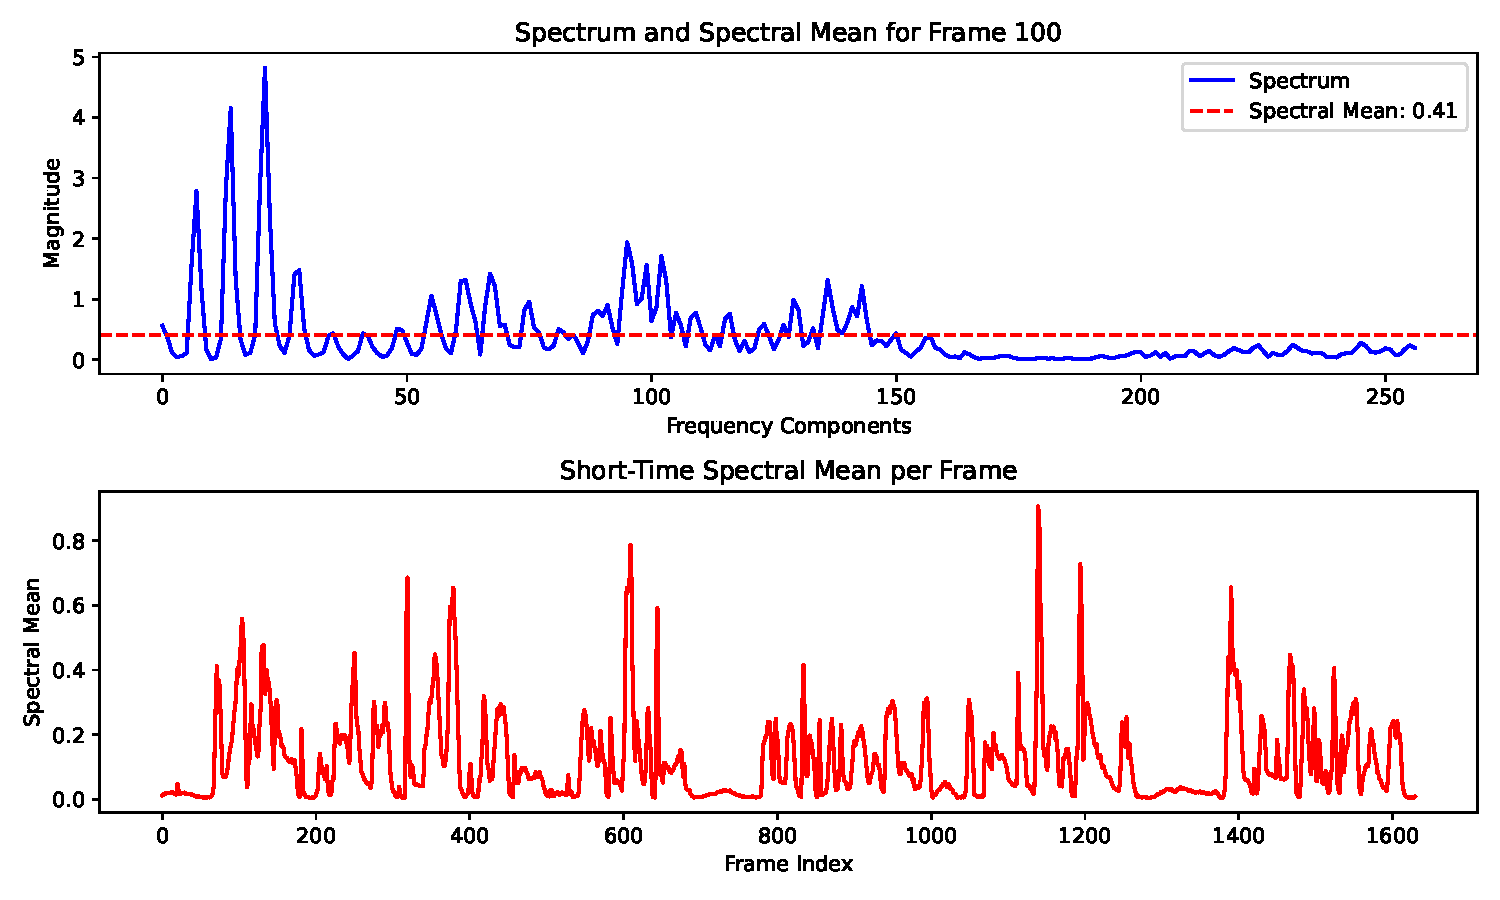
\includegraphics[width=0.5\textwidth]{figs/spectral_mean.pdf}
      \caption{频谱均值}
      \label{fig:spectral mean}
    \end{figure}
    我取出了开发集中的一段语音信号,进行帧长和帧移分别为$512, 128$的分帧,分别求取每一帧的频谱均值,
    并取出第$100$帧的幅度谱与频谱均值,得到图\ref{fig:spectral mean}
  }
\end{enumerate}

\subsubsection{短时子带能量}
\begin{enumerate}
  \item 
  {
    描述:

    子带能量(Subband Energy)是一种将信号频谱分割成若干个频率子带后,对每个子带的能量进行计算的特征。

    大多数信号,特别是语音和音频信号,具有非均匀的频谱分布。
    不同频率的成分对信号的表达有不同的贡献,且在不同的时间段、音节或词汇中,频谱的形态会发生变化。
    因此,将频谱划分为不同的子带,可以帮助我们更细致地分析和提取每个频段的信息。
  }
  \item 
  {
    给人耳听觉的直观感受:
    \begin{itemize}
      \item 子带能量反映了语音信号中不同频率范围的贡献。高频子带能量较强时,语音听起来会更尖锐、清晰

      \item 低频子带能量较强时,语音听起来通常会更加温暖、低沉,例如元音的低频部分
      
      \item 通过分析不同子带的能量,可以得到更精细的音色特征。例如,情感语音中不同的子带能量变化会给人不同的情感感知,如喜悦、愤怒或悲伤
    \end{itemize}
  }
  \item
  {
    可视化与参数选择:

    我取出了开发集中的一段语音信号,使用帧长和帧移分别为$512,128$进行分帧,取出第$100$帧,进行短时傅里叶变换,得到频谱,
    并进行不同数量的子带划分,得到图\ref{fig:subband_energies}:
    \begin{figure}[H]
      \centering
      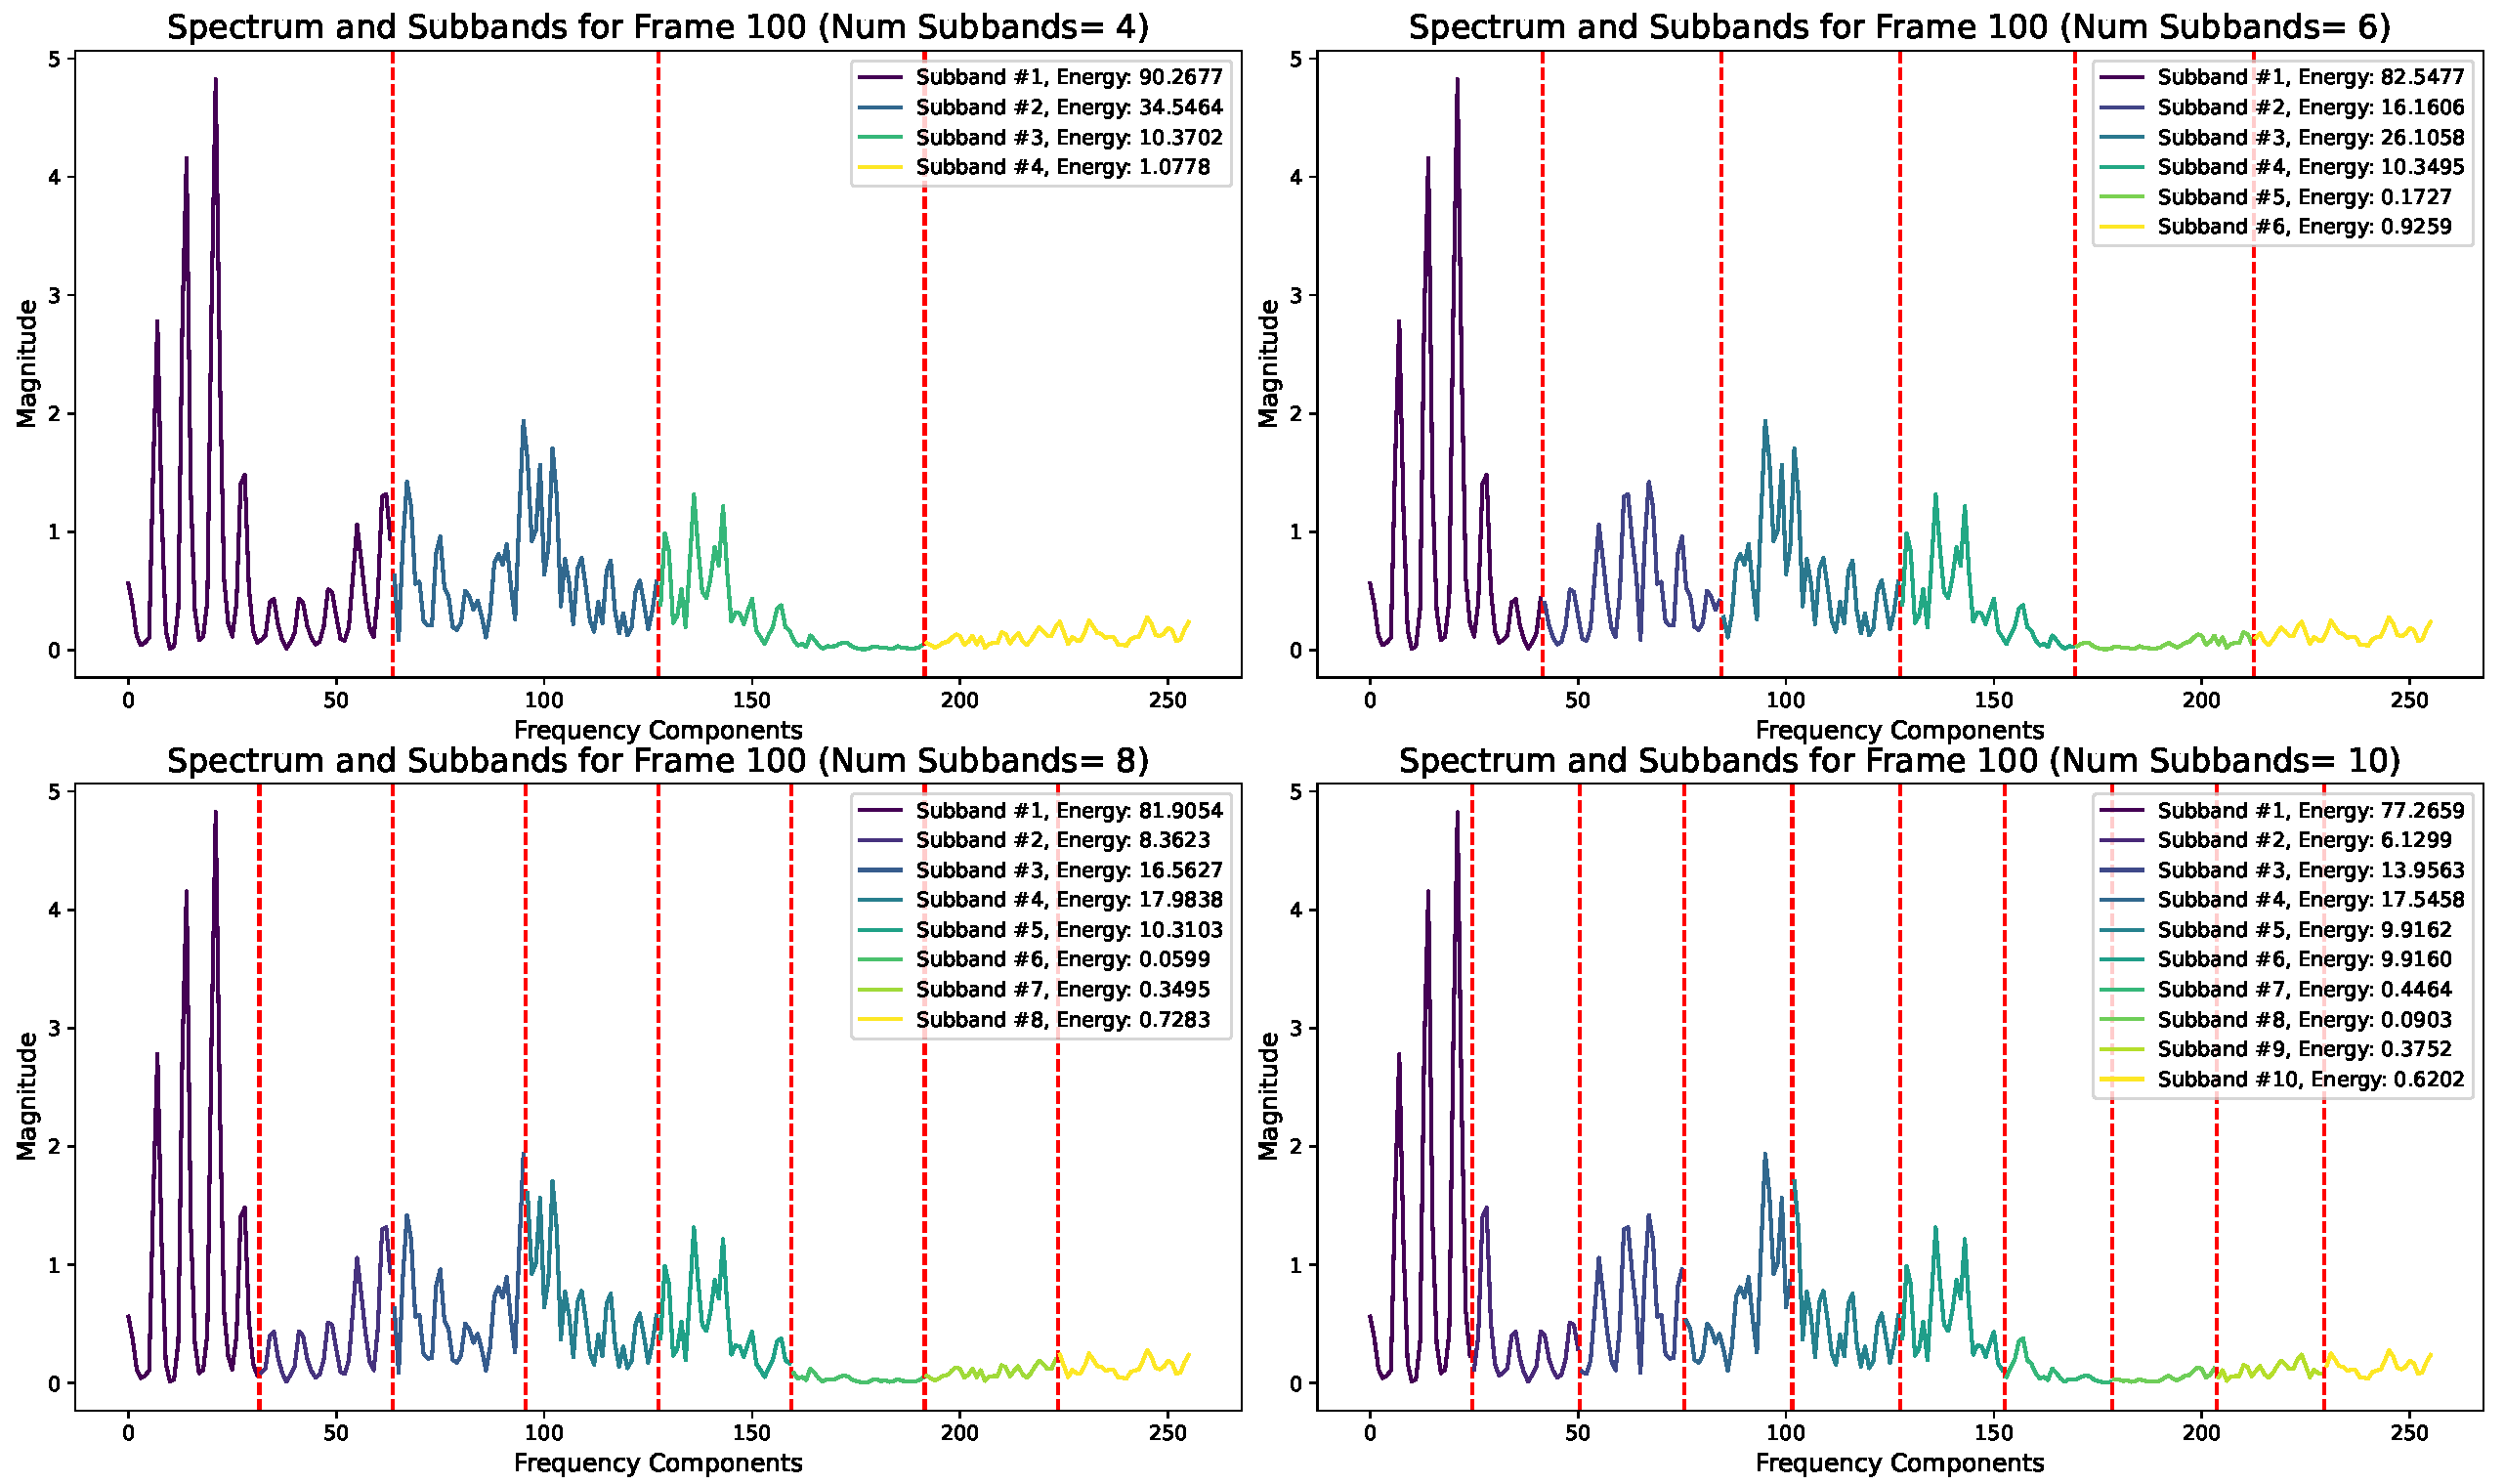
\includegraphics[width=0.5\textwidth]{figs/subband_energies.pdf}
      \caption{子带能量}
      \label{fig:subband_energies}
    \end{figure}
    子带数量选择的好坏,直接与频率分量数目有关系,这又与分帧参数有关。
    为保持一致性,后续实验中,我统一设置\emph{子带数量}为\emph{$6$}。
  }
\end{enumerate}

\subsection{算法描述}

\subsubsection{算法执行流程}
以下是我的算法的执行流程:
\begin{enumerate}
  \item 确定\emph{frame\_size}和\emph{frame\_shift}
  \item 对于训练数据集\emph{dev},获取每一段语音的逐帧标签
  \item 
  {
    对于一段语音信号:
    \begin{enumerate}
      \item \emph{预加重}和\emph{分帧}
      \item 逐帧提取\emph{短时能量}和\emph{短时过零率}以及\emph{短时基频}
      \item 逐帧进行\emph{短时傅里叶变换(STFT)}
      \item 提取\emph{短时频谱均值}和\emph{短时子带能量}这两个频域特征
    \end{enumerate}
  }
  \item 对于训练数据,拼接所有帧的特征以及标签得到$X$和$y$,训练一个\emph{二分类}分类器$F(x)$
  \item 执行预测任务时,对语音信号进行同样的处理,得到逐帧特征$x$,并使用$F$进行预测逐帧标签,并还原出时域的分点
\end{enumerate}

\subsubsection{描述}

在任务一中,首先确定\emph{frame\_size}和\emph{frame\_shift},$i.e.$每一帧在时域中的帧长和帧移,单位为$ms$。

对于开发集\emph{dev},使用\emph{vad\_utils.py}中给出的函数\emph{read\_label\_from\_file},得到每一段语音的逐帧标签。

对于一段语音信号,我首先对其进行\emph{预加重}和\emph{分帧},然后逐帧提取\emph{短时能量}和\emph{短时过零率}这两个时域特征以及\emph{短时基频},
后面逐帧进行\emph{短时傅里叶变换(STFT)},并利用STFT的结果,提取\emph{短时频谱均值}和\emph{短时子带能量}这两个频域特征。

将所有开发集中的语音信号的逐帧特征与逐帧标签拼接起来得到数据特征$X$和标签$y$,
进行训练集和验证集$4: 1$的划分,分别使用\emph{sklearn.StandardScaler()}进行标准化,
然后使用训练数据集训练得到一个\emph{二分类分类器}$F(x)$。

执行预测任务时,对语音信号进行同样的处理,得到逐帧特征$x$,并使用$F$进行预测逐帧标签,
再使用\emph{vad\_utils.py}中给出的函数\emph{prediction\_to\_vad\_label},还原出时域的分点。

\subsubsection{分类器}
在任务一中,我使用了两种分类器:
\begin{itemize}
  \item \emph{Linear SVM}
  \item \emph{Logistic Regression}
\end{itemize}

\subsubsection{特征维度}
我在进行特征提取时得到的各个特征的维度分别为:
  \begin{itemize}
    \item \emph{短时能量}:$1$
    \item \emph{短时过零率}:$1$
    \item \emph{短时基频}:$1$
    \item \emph{短时频谱中心}:$1$
    \item \emph{短时子带能量}:$6$
  \end{itemize}
  因此,输入的特征维度为$10$

\subsection{实验结果}
\subsubsection{各项性能表征}
在本次作业中,我主要考虑的参数是帧长与帧移,我开发集\emph{dev}中的语音逐帧提取出特征与标签后,
按帧全部拼接到一起,然后进行训练集和验证集$4: 1$的划分,分别使用\emph{sklearn.StandardScaler()}进行标准化,然后尝试使用不同的帧长帧移组合,训练不同的分类器,
并观察在验证集上的各项性能。

使用\emph{Linear SVM},得到下面表\ref{tab:Linear SVM}中的数据以及对应的\emph{ROC}曲线(图\ref{fig:ROC Linear SVM})
\begin{table*}[ht]
  \caption{Linear SVM 分类效果}
  \label{tab:Linear SVM}
  \centering
  \begin{tabular}{c|c|c|c|c|c|c|c}
    \toprule
    \textbf{Frame Length} & \textbf{Frame Shift} & \textbf{Accuracy} & \textbf{AUC} & \textbf{EER} & \textbf{Precision} & \textbf{Recall} & \textbf{F1 Score}\\
    \midrule
    320 & 80 & 0.8879 & 0.9376 & 0.1198 & 0.9300 & 0.9330 & 0.9315 \\
    512 & 128 & 0.8937 & 0.9413 & 0.1170 & 0.9349 & 0.9352 & 0.9350 \\
    1024 & 256 & 0.9107 & 0.9534 & 0.1006 & 0.9486 & 0.9419 & 0.9453 \\
    2048 & 512 & 0.9357 & 0.9698 & 0.0780 & 0.9667 & 0.9545 & 0.9606 \\
    4096 & 1024 & \textbf{0.9480} & 0.9765 & \textbf{0.0690} & \textbf{0.9715} & 0.9650 & \textbf{0.9683} \\
    320 & 160 & 0.8890 & 0.9376 & 0.1196 & 0.9309 & 0.9337 & 0.9323 \\
    512 & 256 & 0.8933 & 0.9405 & 0.1190 & 0.9343 & 0.9349 & 0.9346 \\
    1024 & 512 & 0.9101 & 0.9543 & 0.0990 & 0.9478 & 0.9412 & 0.9445 \\
    2048 & 1024 & 0.9346 & 0.9693 & 0.0841 & 0.9666 & 0.9534 & 0.9599 \\
    4096 & 2048 & 0.9479 & \textbf{0.9770} & 0.0700 & 0.9701 & \textbf{0.9661} & 0.9681 \\
    \bottomrule
  \end{tabular}
\end{table*}

\begin{figure}[H]
  \centering
  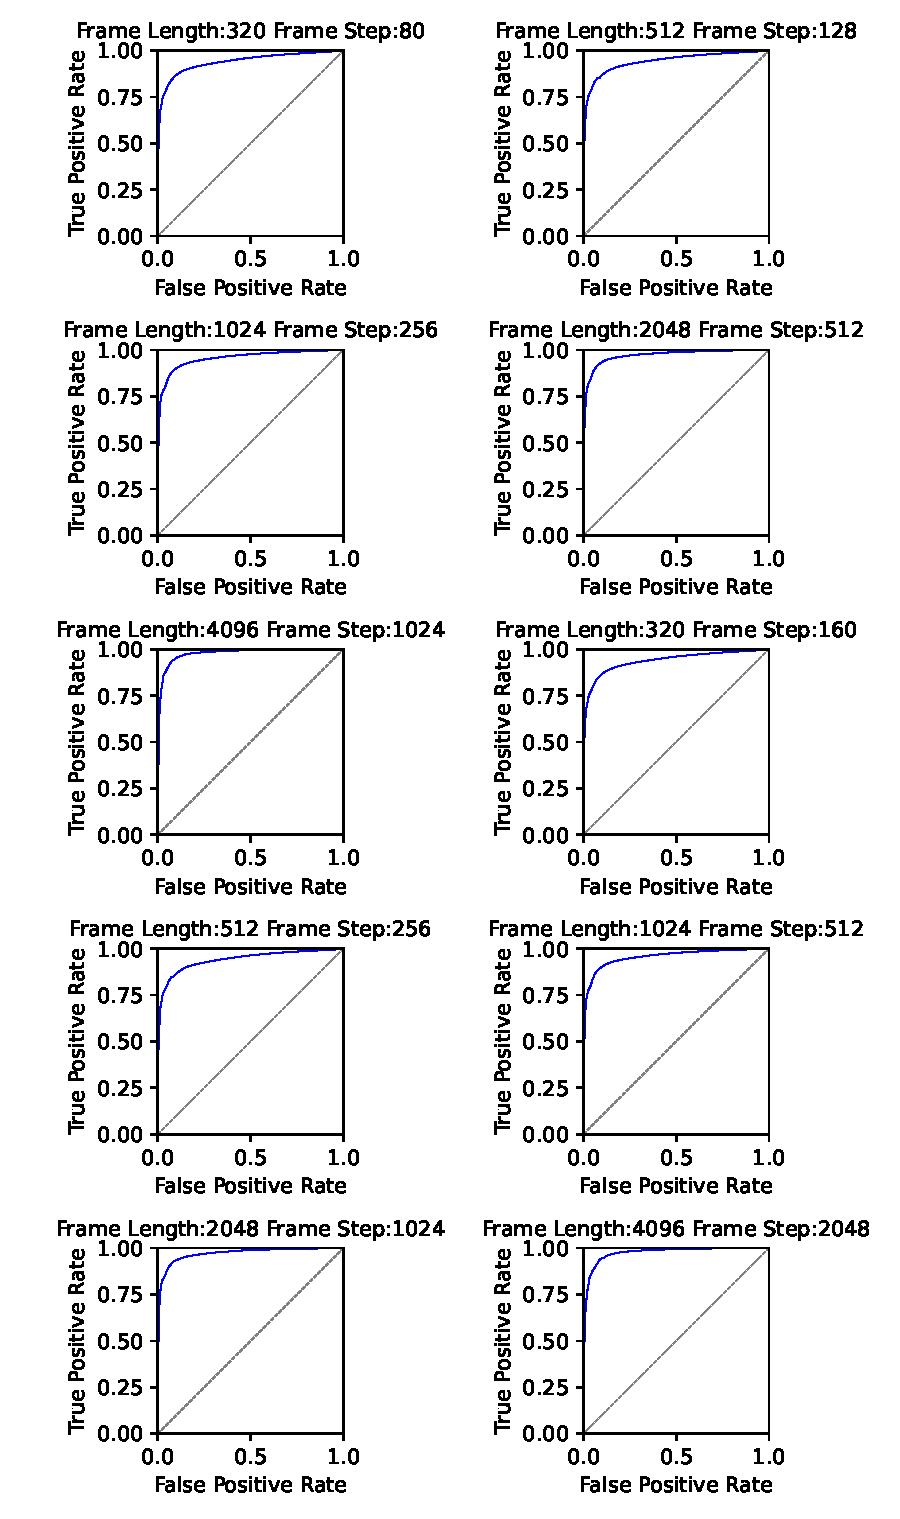
\includegraphics[width=0.5\textwidth]{figs/ROC_Linear_SVM.pdf}
  \caption{不同分帧方法下使用\emph{Linear SVM}的ROC曲线}
  \label{fig:ROC Linear SVM}
\end{figure}


使用\emph{Logistic Regression},得到下面表\ref{tab:Logistic Regression}中的数据以及对应的\emph{ROC}曲线(图\ref{fig:ROC Logistic Regression})
\begin{table*}[ht]
  \caption{Logistic Regression 分类效果}
  \label{tab:Logistic Regression}
  \centering
  \begin{tabular}{c|c|c|c|c|c|c|c}
    \toprule
    \textbf{Frame Length} & \textbf{Frame Shift} & \textbf{Accuracy} & \textbf{AUC} & \textbf{EER} & \textbf{Precision} & \textbf{Recall} & \textbf{F1 Score}\\
    \midrule
    320 & 80 & 0.8952 & 0.9407 & 0.1206 & 0.9371 & 0.9346 & 0.9358 \\
    512 & 128 & 0.9008 & 0.9457 & 0.1134 & 0.9432 & 0.9347 & 0.9389 \\
    1024 & 256 & 0.9174 & 0.9589 & 0.0974 & 0.9544 & 0.9443 & 0.9493 \\
    2048 & 512 & 0.9405 & 0.9734 & 0.0763 & 0.9687 & 0.9586 & 0.9636 \\
    4096 & 1024 & 0.9460 & \textbf{0.9763} & 0.0758 & 0.9697 & 0.9648 & 0.9673 \\
    320 & 160 & 0.8946 & 0.9405 & 0.1204 & 0.9369 & 0.9342 & 0.9355 \\
    512 & 256 & 0.9020 & 0.9460 & 0.1123 & 0.9436 & 0.9358 & 0.9396 \\
    1024 & 512 & 0.9176 & 0.9591 & 0.0968 & 0.9536 & 0.9449 & 0.9492 \\
    2048 & 1024 & 0.9353 & 0.9705 & 0.0809 & 0.9649 & 0.9553 & 0.9601 \\
    4096 & 2048 & \textbf{0.9490} & 0.9757 & \textbf{0.0719} & \textbf{0.9719} & \textbf{0.9659} & \textbf{0.9689} \\
    \bottomrule
  \end{tabular}
\end{table*}

\begin{figure}[ht]
  \centering
  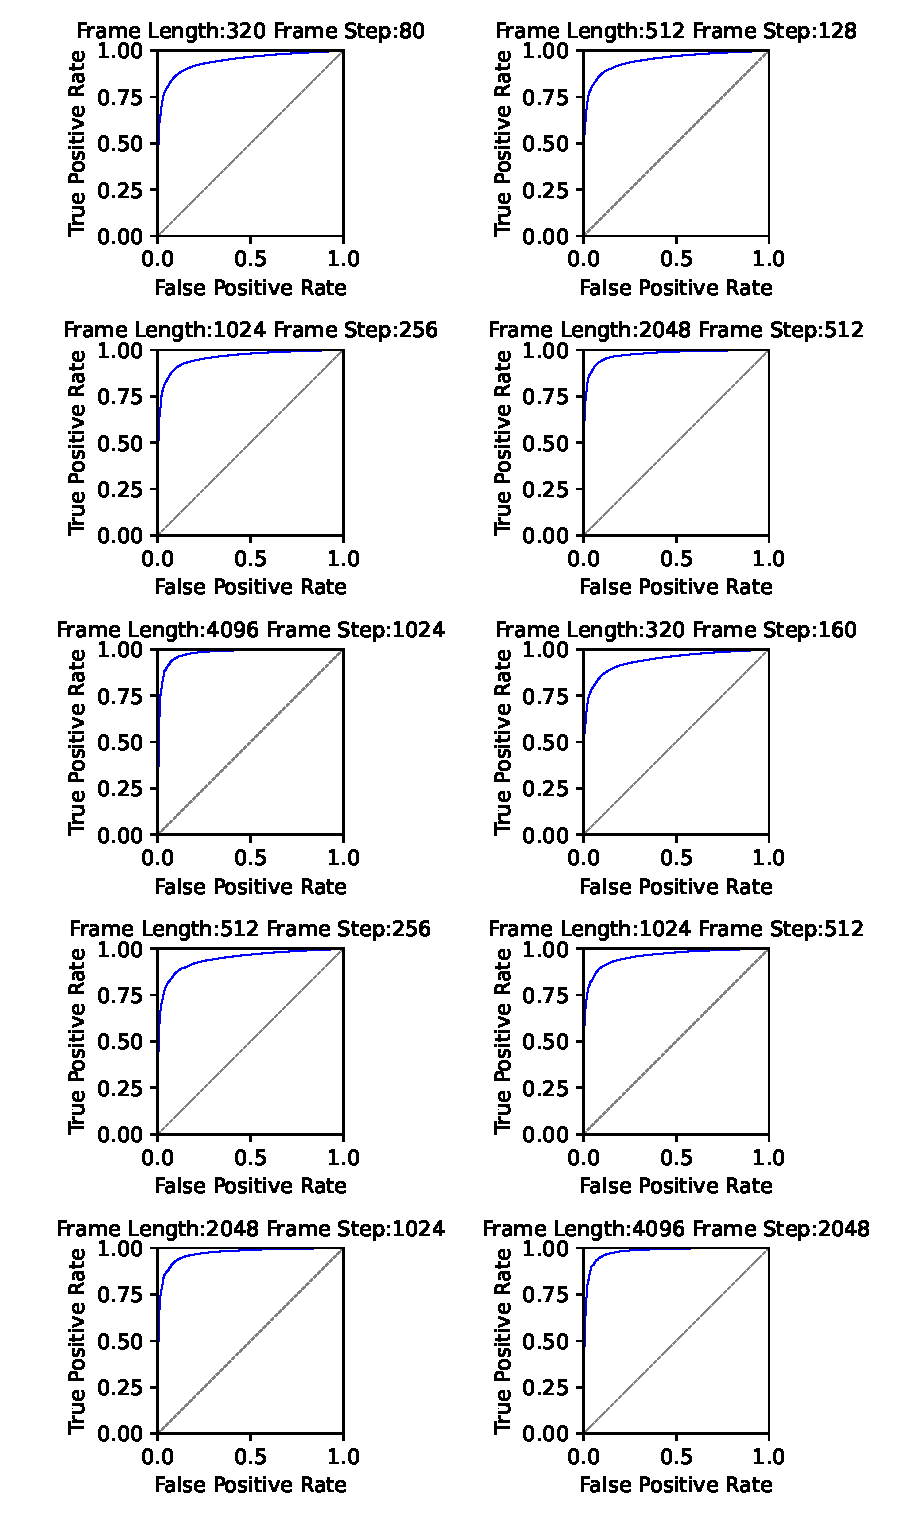
\includegraphics[width=0.5\textwidth]{figs/ROC_Logistic_Regression.pdf}
  \caption{不同分帧方法下使用\emph{Logistic Regression}的ROC曲线}
  \label{fig:ROC Logistic Regression}
\end{figure}

通过观察可以发现,不论是\emph{Linear SVM}还是\emph{Logistic Regression},二分类的性能均会随着帧长的增加而提升,
但是这仅仅说明模型对切分好的帧有较强的分类能力,于是我进行了下面的时域信号切分的可视化。

\subsubsection{可视化}
我取出了开发集中的一段语音信号,并使用不同分帧方法,测试了两种分类器的表现,
得到如图\ref{fig:results Linear SVM}和图\ref{fig:results Logistic Regression}中的效果。
\begin{figure}[H]
  \centering
  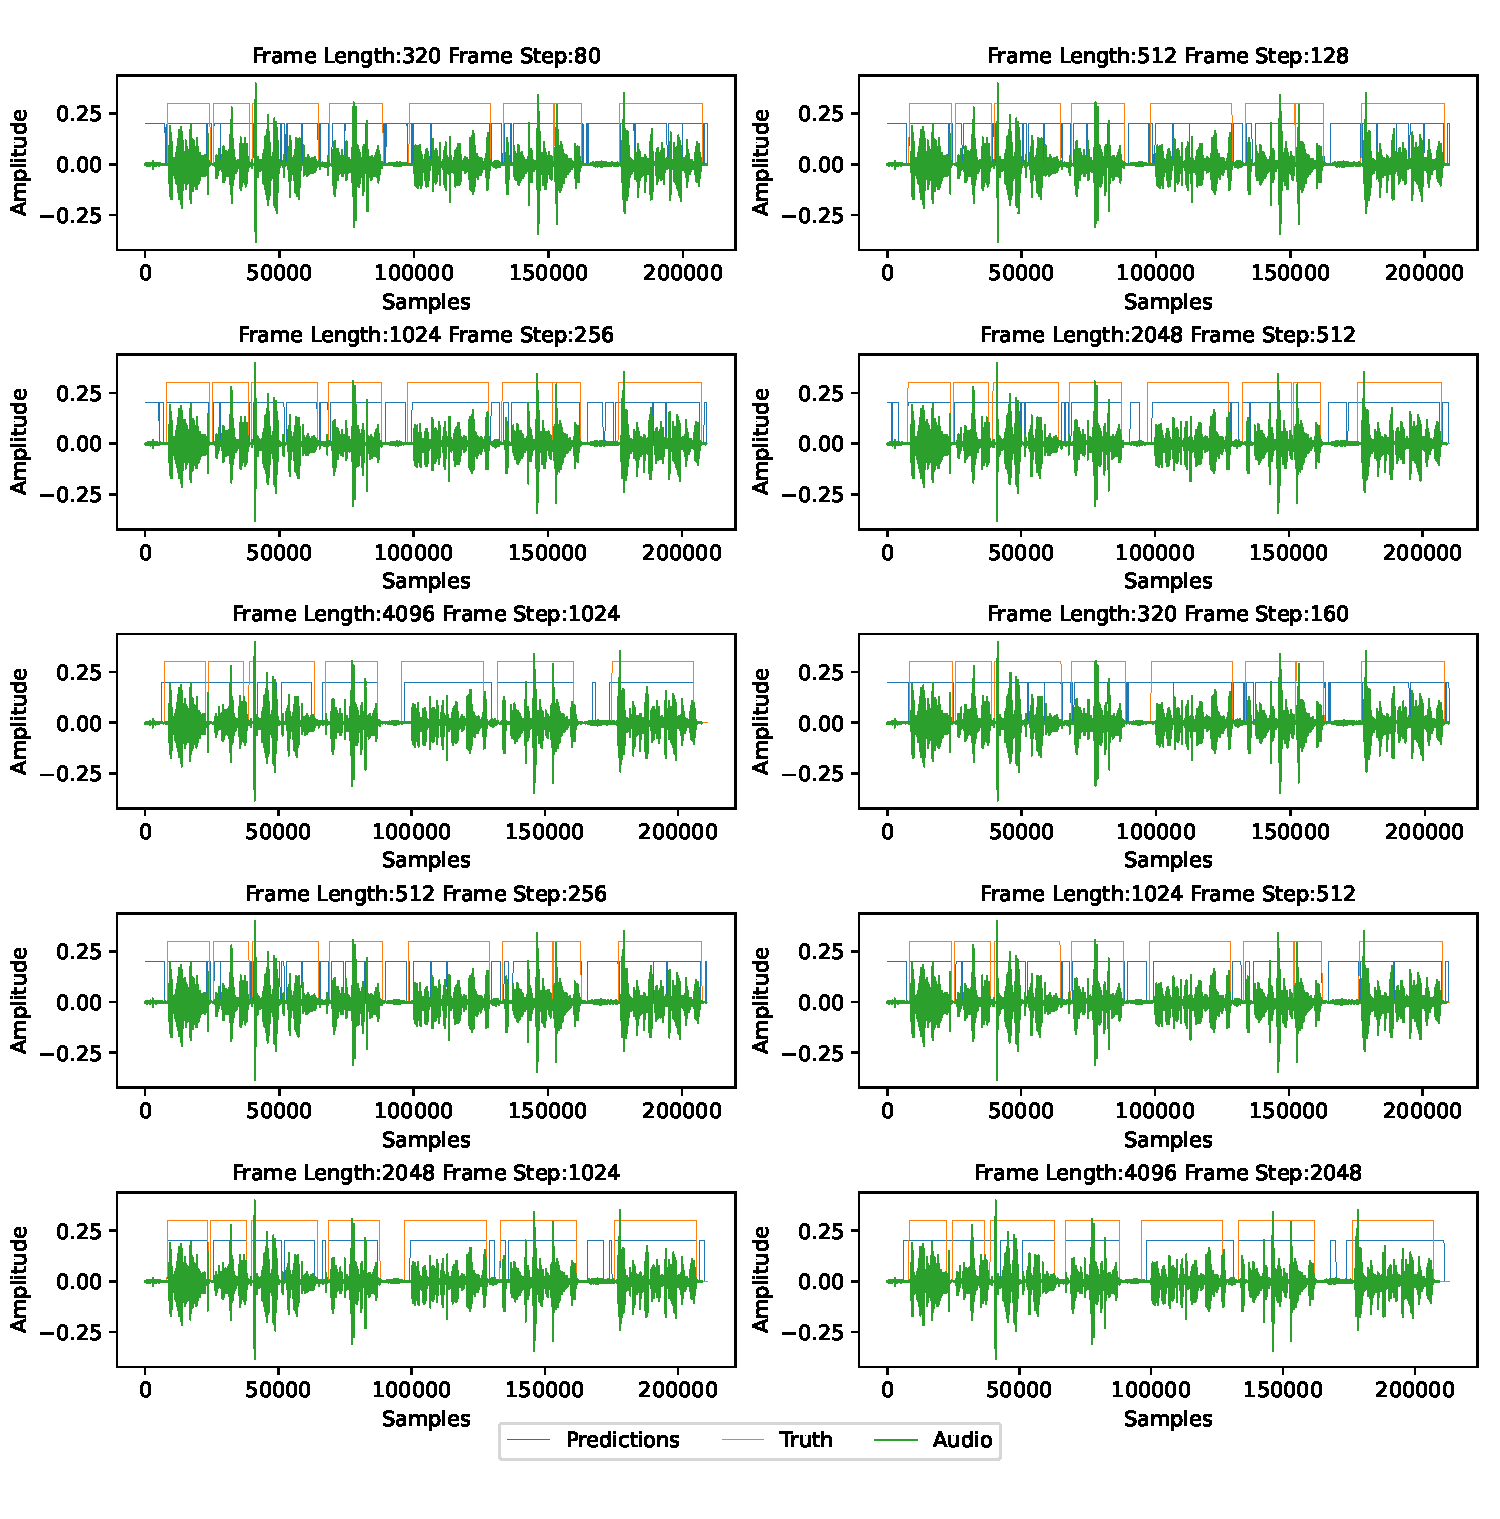
\includegraphics[width=0.5\textwidth]{figs/visualize_results_Linear_SVM.pdf}
  \caption{不同分帧方法下使用\emph{Linear SVM}的表现}
  \label{fig:results Linear SVM}
\end{figure}

\begin{figure}[ht]
  \centering
  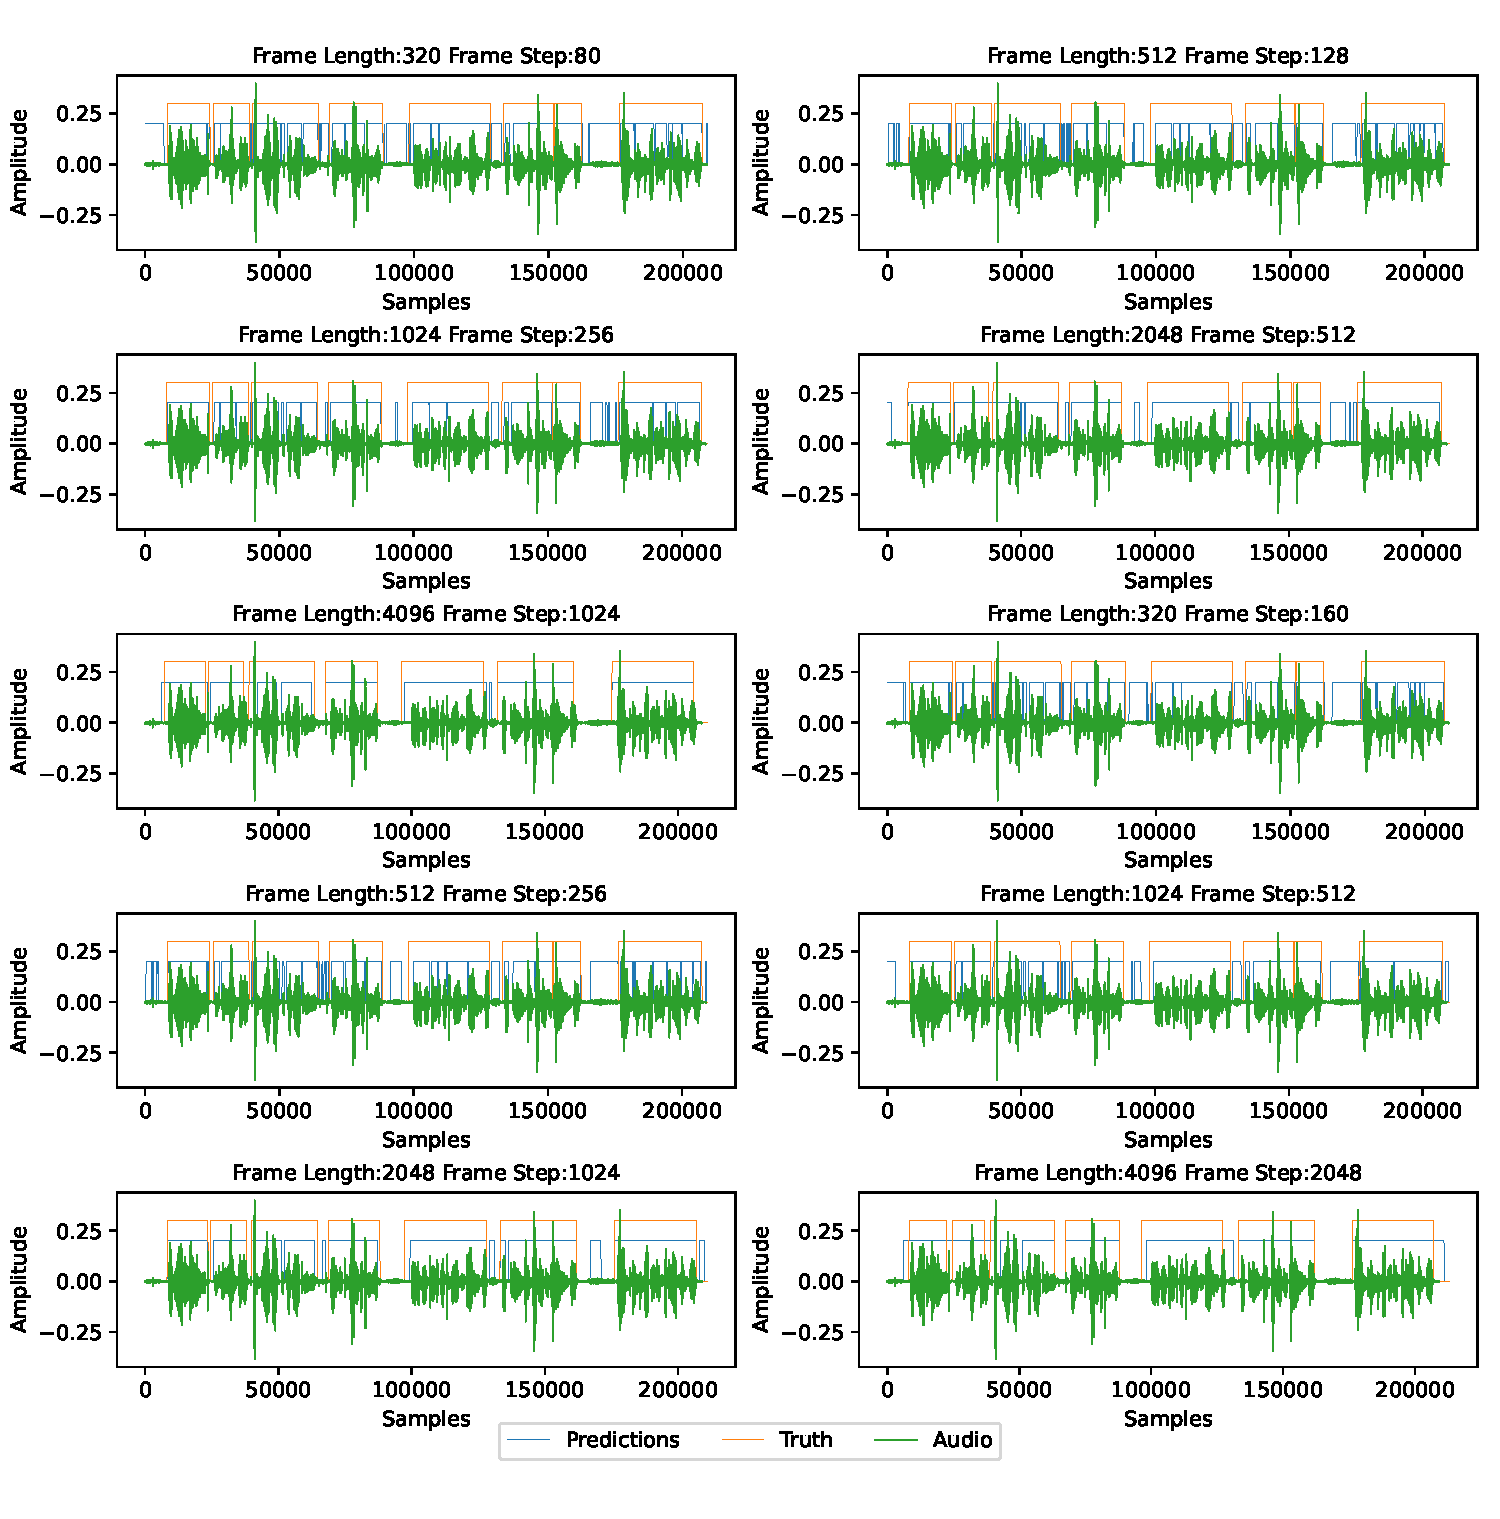
\includegraphics[width=0.5\textwidth]{figs/visualize_results_Logistic_Regression.pdf}
  \caption{不同分帧方法下使用\emph{Logistic Regression}的表现}
  \label{fig:results Logistic Regression}
\end{figure}
其中,绿色线是原始波形图,蓝色线表示预测的语音端点,黄色线表示真实的语音端点。

可以看出,在帧长和帧移都比较小的时候,划分是更加精细的,但是会存在较多的非语音片段被划分为语音片段的情况,
相比之下,在帧长较大时,划分可能更粗犷,在划分边界处会不够精确,但是上述错误会少很多。

\subsubsection{关于实验结果的思考}
下面是我认为的帧长和帧移对\emph{VAD}任务的具体影响:
\begin{enumerate}
  \item 
  {
    帧长:
    \begin{itemize}
      \item 较长的帧长:

      优点: 提供更多的频域信息,适合捕捉较长的语音特征
      
      缺点: 会降低时间分辨率,可能导致端点检测不够精确,尤其在快速语音变化的情况下。也会增加计算负担,因为每一帧处理的数据更多。
      此外,可能导致我们的语音信号在短时内是近似平稳的这个假设不稳固
      \item 较短的帧长:

      优点: 提供更高的时间分辨率,使得端点检测更精确,尤其适用于快速变化的语音信号
      
      缺点: 频域信息较少,可能无法有效捕捉较长的音频特征,噪声对短帧的影响可能更大
    \end{itemize}
  }
  \item 
  {
    帧移:
    \begin{itemize}
      \item 较小的帧移:

      优点: 增加了帧之间的重叠,能够提高时间分辨率,帮助更准确地捕捉语音信号的变化,提高了模型预测的连续性
      
      缺点: 会增加计算量和存储需求,因为计算结果会更密集
      \item 较大的帧移:

      优点: 减少计算量,适用于实时处理
      
      缺点: 会降低时间分辨率,可能导致检测不准确,特别是在语音信号的快速变化或端点的准确定位上
      \item 通常,帧移的大小为帧长的$\frac{1}{2}$到$\frac{1}{4}$
    \end{itemize}
  }
\end{enumerate}

综合考虑,最后的结果我将使用\emph{帧长$4096$}和\emph{帧移$1024$}来进行分帧。

\section{基于统计模型分类器和语音频域特征的语音端点检测算法}

\subsection{数据预处理及特征提取}

在任务二中,我使用的数据预处理操作和任务一中的操作相同,
同样进行\textbf{预加重},\textbf{分帧}以及\textbf{加窗}。

在任务二中,我增加了四项特征:
\begin{itemize}
  \item \textbf{Mel域的FBank系数}
  \item \textbf{MFCC}
  \item \textbf{Delta MFCC}
  \item \textbf{Delta of Delta MFCC}
\end{itemize}

\subsubsection{Mel域的FBank系数}
\begin{enumerate}
  \item 
  {
    描述:

    \emph{Mel scale}是一个基音感知域,它通过听音者可以区分两种纯音频率的差距来作为标度。
    Mel域和线性频域之间通过一个非线性的映射函数
    可以相互转换:
    \begin{equation}
      Mel(f) = 2595\log_{10}(1 + \frac{f}{700})
      \label{eq:Mel Domain}
    \end{equation}
    FBbank(Mel频率倒谱系数)主要作用是通过模拟人类听觉系统的响应来对语音信号进行特征提取,
    从而更好地匹配人类的听觉感知。
  }
  \item 
  {
    效果:
    \begin{itemize}
      \item 频谱压缩:
      
      通过Mel尺度的压缩,FBank降低了高频部分的信息量,这符合人耳对高频信号较弱的敏感度
      \item 增强音频特征:
      
      更好地捕捉语音中与听觉相关的特征,能够有效地过滤掉一些与语音本身无关的噪声
      \item 语音识别性能提高:
      
      由于其能较好地模拟人耳听觉机制,FBank特征在语音识别中能提高系统的性能,尤其是在背景噪音较大的环境之中
    \end{itemize}
  }
  \item 
  {
    给人耳听觉的直观感受:
    \begin{itemize}
      \item 人类的听觉系统对不同频率的声音响应是非线性的,在低频部分能更精细地分辨音高变化,
      而在高频部分分辨率较低。Mel尺度正是基于这种感知特性设计的。
      FBank通过将频率分为多个Mel尺度的带宽,使得每个带宽能模拟人耳对声音的不同感知强度,
      从而提升了语音信号的有效特征。
      \item 从直观感受上,FBank特征提取的信号类似于人耳对语音信号的“感知”表现。
      与传统的线性频率尺度不同,FBank在低频段捕捉到更多细节信息,
      而在高频段则压缩了信息,使得对噪声的鲁棒性增强,同时不损失关键信息。
    \end{itemize}
  }
  \item 
  {
    计算:

    \begin{equation}
      m_i = \sum_{k=f_i}^{F_i}s(k)T_i(k)
      \label{eq:FBank}
    \end{equation}
    其中,$m_i$是第$i$个FBank系数,$f_i$和$F_i$分别是Mel滤波器的开始和结束频率,
    $s(k)$是在频点$k$的谱的能量(有时为谱的幅值,这里我取的能量),$T_i(k)$是Mel滤波器的值。
    \begin{figure}[H]
      \centering
      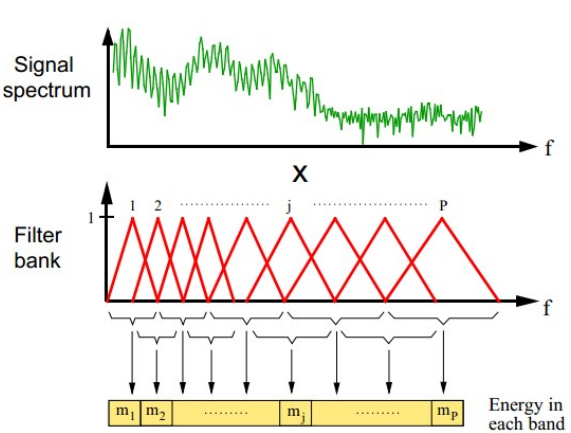
\includegraphics[width=0.5\textwidth]{figs/visualize_FBank.png}
      \caption{FBank计算直观图}
      \label{fig:visualize FBank}
    \end{figure}
  }
  \item 
  {
    代码实现:
    \begin{lstlisting}[language=python]
def Filter_banks(stft: np.ndarray, sampling_rate: int = 16000, frame_lenth: int = 512, num_filters: int = 23):
  filter_banks = []
  mel_filters = librosa.filters.mel(sr=sampling_rate, n_fft=frame_lenth, n_mels=num_filters)
  num_frames = stft.shape[0]
  for i in range(num_frames):
    spectrum = np.abs(stft[i]) ** 2
    f_bank = np.dot(mel_filters, spectrum)
    filter_banks.append(f_bank)
  return np.array(filter_banks)
    \end{lstlisting}

  \begin{enumerate}
    \item 传入参数:STFT频谱矩阵$stft$,采样率$sampling\_rate$,帧长$frame\_length$, 滤波器数量 $num\_filters$
    \item 计算 Mel 滤波器组
    \item 获取 STFT 的帧数
    \item 计算每一帧的幅度谱平方
    \item 通过 Mel 滤波器组计算 FBank 特征
    \item 最后返回FBank系数
  \end{enumerate}
  }
\end{enumerate}

\subsubsection{MFCC}
\begin{enumerate}
  \item 
  {
    描述:

    MFCC是语音信号处理中非常有效且广泛使用的特征,它通过模仿人耳的听觉特性,
    提取了符合人类听觉机制的特征。
  }
  \item 
  {
    效果:
    \begin{itemize}
      \item 模拟人耳感知:
      
      MFCC 的核心特点是模拟了人耳的听觉特性,尤其是 Mel 频率尺度和对数变换的步骤。
      这使得 MFCC 能够有效地反映人类听觉系统对语音信号的感知,从而在语音识别任务中提供更符合实际的特征表示

      \item 降维与特征提取:
      
      通过\emph{DCT}压缩了信息量,去除了冗余的特征。通常,MFCC特征维度较低(通常为$13$维左右,此处我默认设置为$12$维),
      这有助于减轻后续模型的计算负担,同时保留了足够的语音信息
      
      提高语音识别性能:
      
      由于其模拟了人耳的感知机制,MFCC在语音识别任务中通常表现得比原始的频谱特征更好,尤其在有噪声或环境变化时
    \end{itemize}
  }
  \item 
  {
    给人耳听觉的直观感受:

    从直观上看,MFCC 特征通过 Mel 滤波器组和对数变换,有效地模拟了人耳对声音强度和频率的感知:
    \begin{itemize}
      \item 在低频段,它能细致地捕捉语音的音高和语调变化。
      \item 在高频段,尽管信息较少,但仍能保留足够的语音识别相关特征,比如清晰度和音色。
    \end{itemize}
    
    简而言之,MFCC 特征在音频信号处理中的优势在于其能够模拟人耳对语音信号的响应方式,从而使语音识别和其他语音处理任务更加符合人类的听觉感知。
  }
  \item 
  {
    计算:

    \begin{enumerate}
      \item 取对数logarithm得到$N$个对数域的FBank系数
      \item 计算倒谱Cepstral系数,使用 Discrete Cosine Transform(DCT)变换
    \end{enumerate}

    \begin{equation}
      \begin{split}
          c_n &= \sqrt{\frac{2}{N_{fb}}}\sum_{j=1}^{N_{fb}}\log(m_j)\cos\left(\frac{\pi n}{N_{fb}}\left(j - 0.5\right)\right) \\
          n &= 1, 2, \dots, N_{mfcc}
          \label{eq:MFCC}
      \end{split}
  \end{equation}
  }
  \item 
  {
    代码实现:
    \begin{lstlisting}[language=python]
def Mfcc(f_banks: np.ndarray, num_mfcc: int =12):
  f_banks = np.where(f_banks == 0, np.finfo(float).eps, f_banks) # 数值稳定性
  log_mel = 10 * np.log10(f_banks)
  mfcc = dct(log_mel, type=2, axis=1, norm="ortho")
  mfcc = mfcc[:, :num_mfcc]
  return mfcc
    \end{lstlisting}
    \begin{enumerate}
      \item 传入参数:FBanks系数以及MFCC系数数量
      \item 处理零值,确保数值稳定性
      \item 计算 Mel 滤波器组的对数能量
      \item 对对数 Mel 能量谱应用离散余弦变换(DCT),
      同\emph{librosa}库中的实现一样,
      \emph{dct}的\emph{norm}参数设置为\emph{"ortho"},并保留前 $num\_mfcc$ 个系数
      \item 最后返回 MFCC 特征矩阵
    \end{enumerate}
  }

  \item 
  {
    可视化:
    \begin{figure}[H]
      \centering
      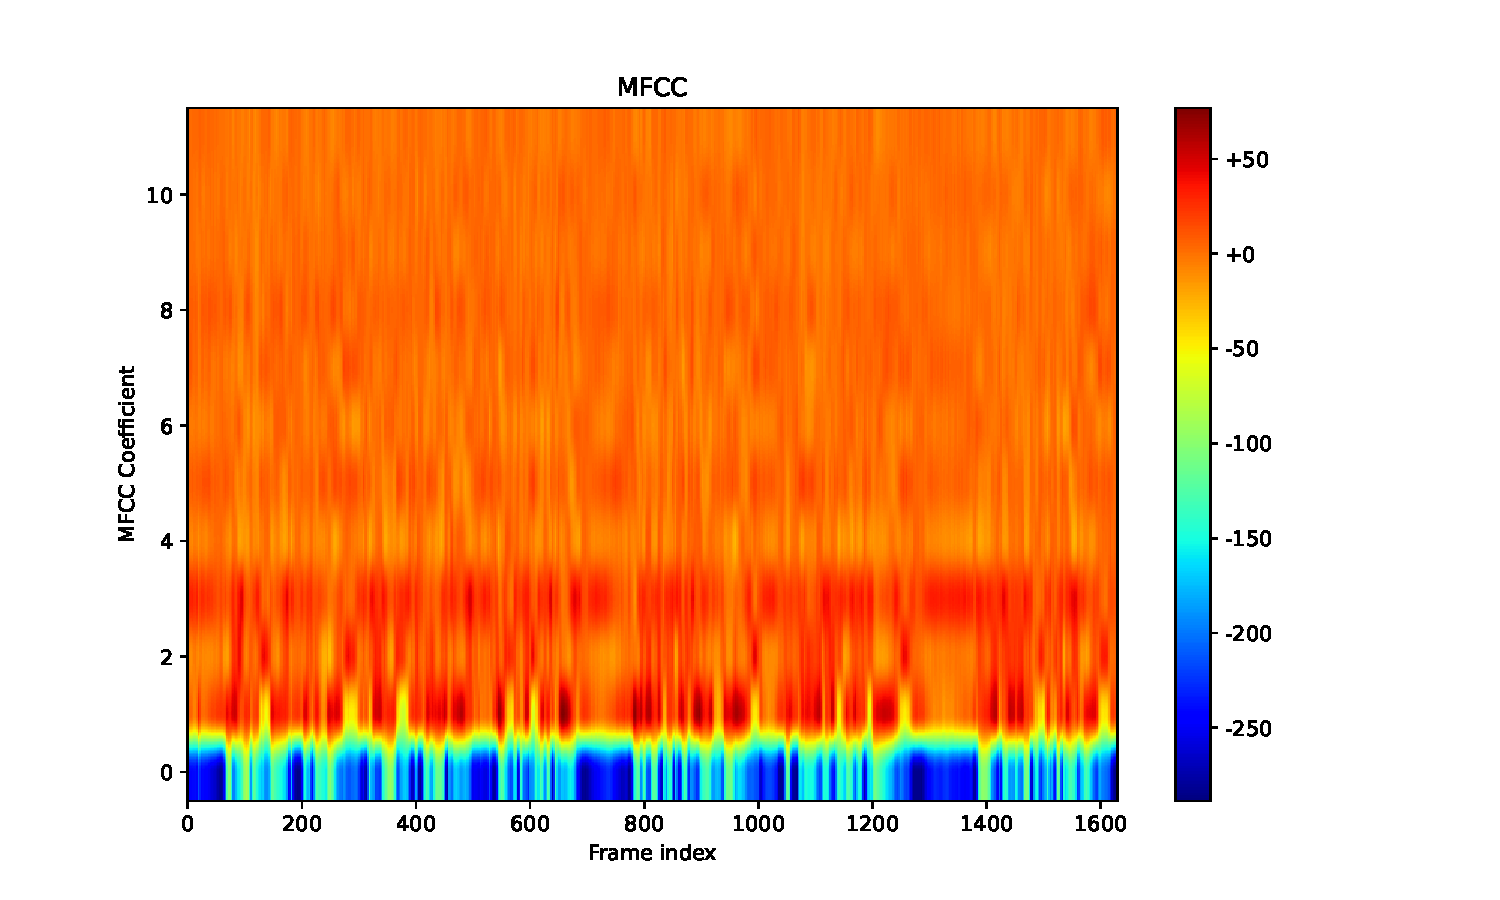
\includegraphics[width=0.5\textwidth]{figs/visualize_MFCC.pdf}
      \caption{MFCC}
      \label{fig:MFCC}
    \end{figure}
  }
\end{enumerate}

\subsubsection{Delta MFCC以及Delta of Delta MFCC}
\begin{enumerate}
  \item 
  {
    描述:

    MFCC 特征很好地描述了即时语音信号谱(静态),但是不能描述信号的动态特性。
    这个不足可以通过在特征向量中添加静态系数的差分特征来得到改善。
  }
  \item 
  {
    计算:
    \begin{itemize}
      \item 简单的差分计算如下:
      \begin{equation}
        \Delta_n = \frac{c_{n+\delta} - c_{n-\delta}}{2\delta}
        \label{eq:Delta1}
      \end{equation}
      \item 更鲁棒的估计是通过一系列语音帧的最佳线性回归系数来得到:(这里是 $2\sigma + 1$)
      \begin{equation}
        \Delta_n = \frac{\sum_{i=1}^{\delta} i (c_{n+i} - c_{n-i})}{2 \sum_{i=1}^{\delta} i^2}
        \label{eq:Delta2}
      \end{equation}
  
      \item 更高阶的差分系数可以通过以上过程的迭代形式来获得:
      \begin{equation}
        \Delta \Delta_n = \frac{\sum_{i=1}^{\delta} i (\Delta_{n+i} - \Delta_{n-i})}{2 \sum_{i=1}^{\delta} i^2}
        \label{eq:delta of delta}
      \end{equation}
  \end{itemize}
  }
  \item 
  {
    代码实现:
    \begin{lstlisting}[language=python]
def weighted_difference(features, delta=1):
  num_frames, num_coeffs = features.shape
  delta_features = np.zeros_like(features)
  weights = np.array([i for i in range(1, delta + 1)])
  weight_sum = np.sum(weights**2)
      
  for t in range(delta, num_frames - delta):
    for f in range(num_coeffs):
      delta_features[t, f] = np.sum(weights * (mfcc[t + np.arange(1, delta + 1), f] - features[t - np.arange(1, delta + 1), f])) / weight_sum
      
  return delta_features
    \end{lstlisting}
    \begin{enumerate}
      \item 传入参数:需要做差分的特征,可以是\emph{MFCC}或者\emph{Delta of MFCC},
      以及窗口大小$\delta$,我这里设置为$1$
      \item 返回:差分后的特征
    \end{enumerate}
  }
  \item 
  {
    可视化:
    \begin{figure}[H]
      \centering
      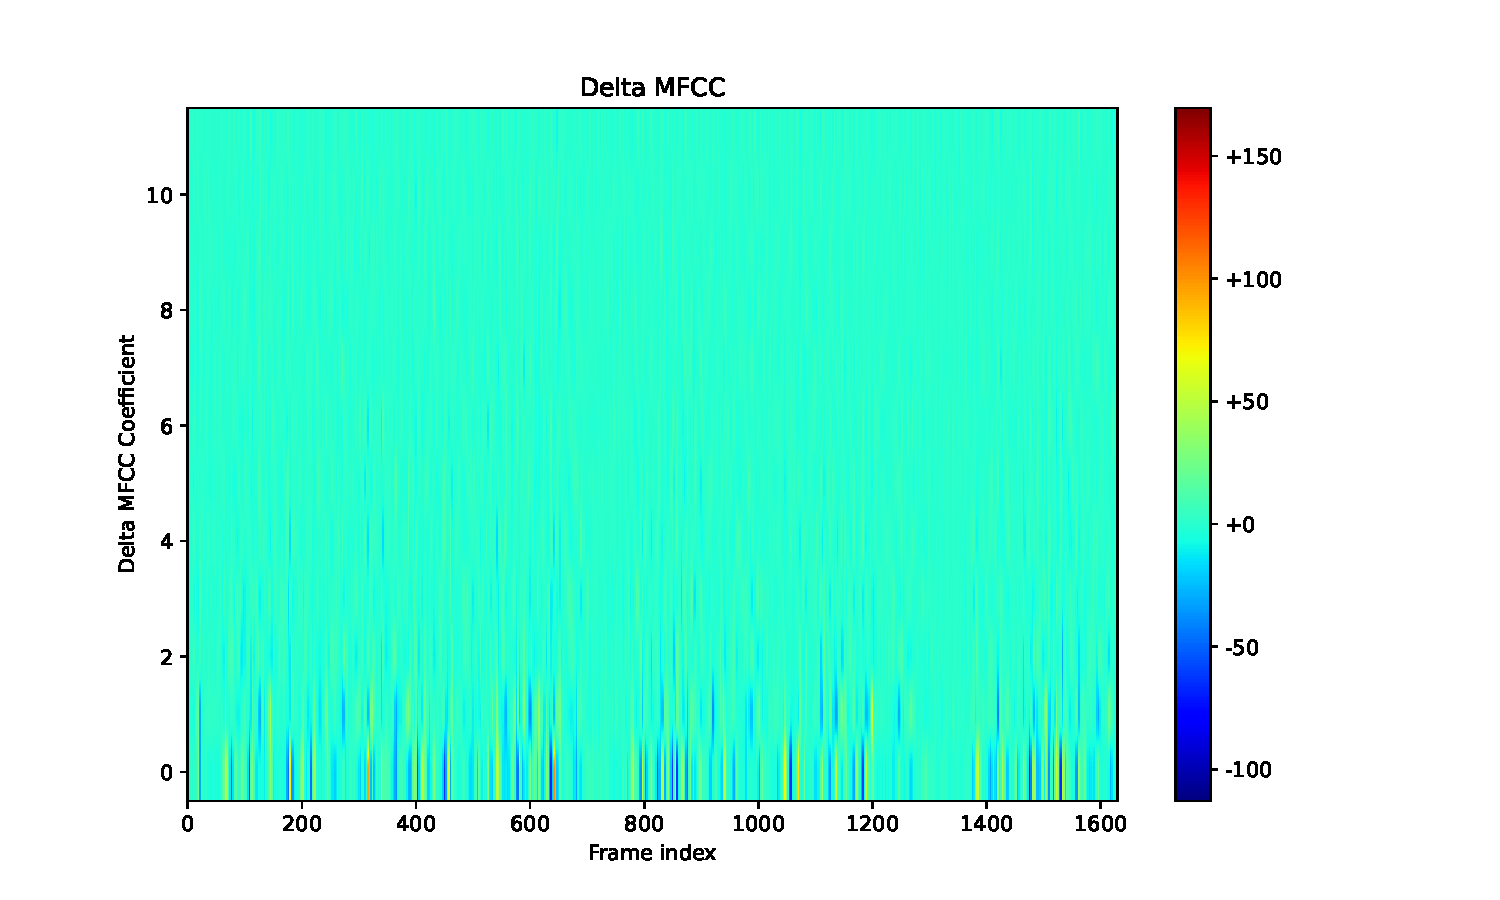
\includegraphics[width=0.5\textwidth]{figs/visualize_Delta_MFCC.pdf}
      \caption{Delta MFCC}
      \label{fig:Delta MFCC}
    \end{figure}
    \begin{figure}[H]
      \centering
      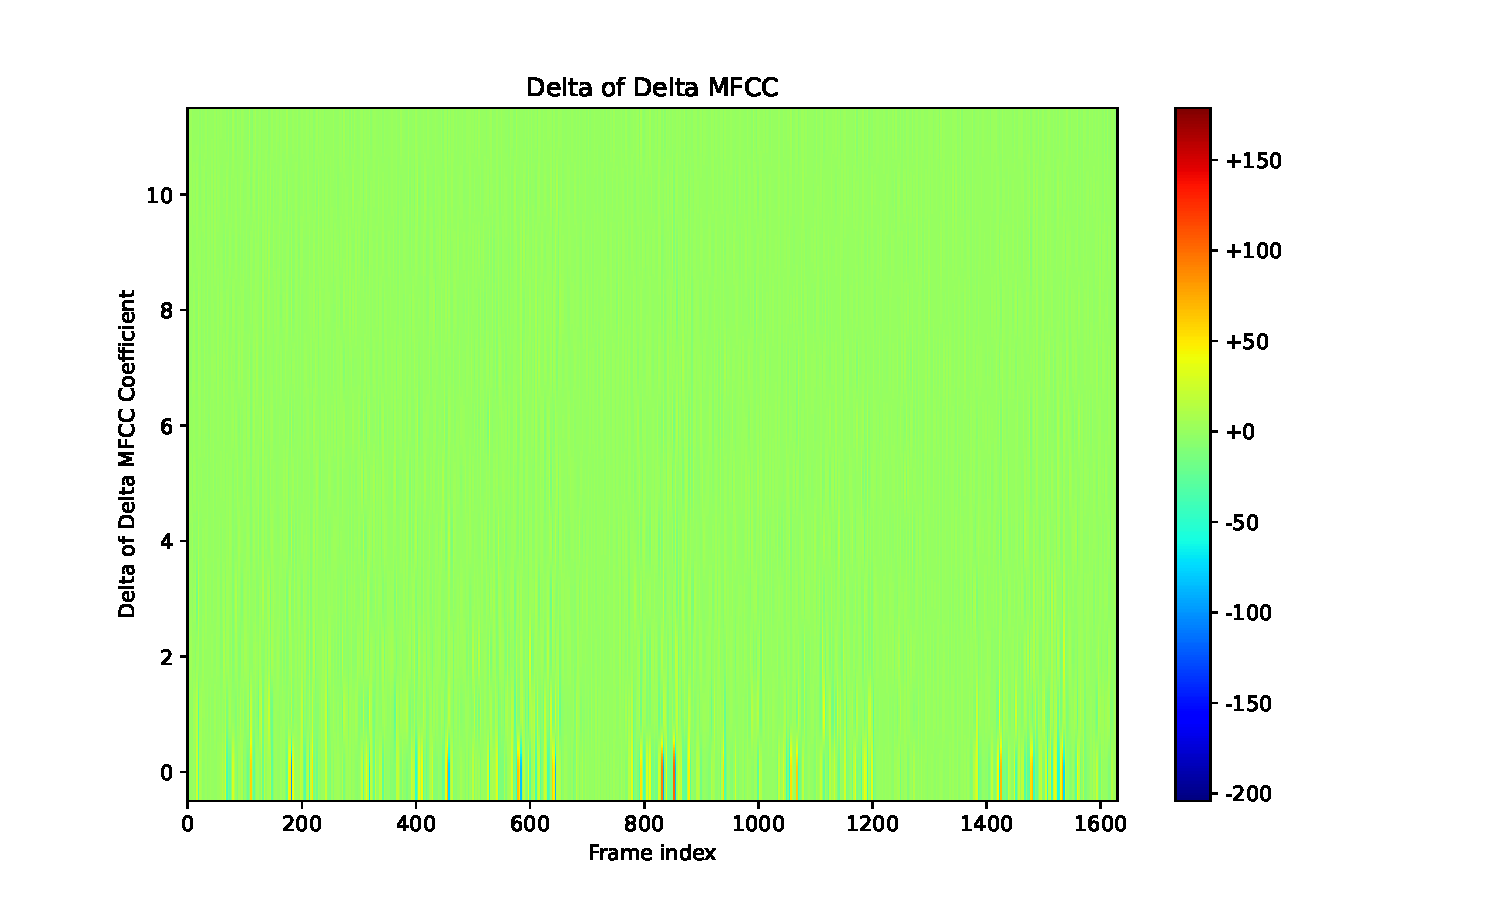
\includegraphics[width=0.5\textwidth]{figs/visualize_Delta_of_Delta_MFCC.pdf}
      \caption{Delta of Delta MFCC}
      \label{fig:Delta of Delta MFCC}
    \end{figure}

  }
\end{enumerate}


\subsection{算法描述}

\subsubsection{算法执行流程}
以下是我的算法的执行流程:
\begin{enumerate}
  \item 确定\emph{frame\_size}和\emph{frame\_shift}
  \item 对于训练数据集\emph{train},获取每一段语音的逐帧标签
  \item 
  {
    对于一段语音信号:
    \begin{enumerate}
      \item \emph{预加重}和\emph{分帧}
      \item 逐帧提取\emph{短时能量}和\emph{短时过零率}以及\emph{短时基频}
      \item 逐帧进行\emph{短时傅里叶变换(STFT)}
      \item 提取\emph{短时频谱均值}和\emph{短时子带能量}这两个频域特征
      \item 提取\emph{Fbanks},\emph{MFCC},\emph{Delta MFCC}以及\emph{Delta of Delta MFCC}
    \end{enumerate}
  }
  \item 对于训练数据,拼接所有帧的特征以及标签得到$X$和$y$,训练一个\emph{二分类}分类器$F(x)$
  \item 执行预测任务时,对语音信号进行同样的处理,得到逐帧特征$x$,并使用$F$进行预测逐帧标签,并还原出时域的分点
\end{enumerate}

\subsubsection{描述}

在任务二中,首先确定\emph{frame\_size}和\emph{frame\_shift},$i.e.$每一帧在时域中的帧长和帧移,单位为$ms$。

对于训练数据集\emph{train},使用\emph{vad\_utils.py}中给出的函数\emph{read\_label\_from\_file},得到每一段语音的逐帧标签。

对于一段语音信号,我首先对其进行\emph{预加重}和\emph{分帧},然后逐帧提取\emph{短时能量}和\emph{短时过零率}这两个时域特征以及\emph{短时基频},
后面逐帧进行\emph{短时傅里叶变换(STFT)},并利用STFT的结果,提取\emph{短时频谱均值}和\emph{短时子带能量}这两个频域特征,提取\emph{Fbanks},\emph{MFCC},\emph{Delta MFCC}以及\emph{Delta of Delta MFCC}。

将训练数据集\emph{train}中的语音信号的逐帧特征与逐帧标签拼接起来得到数据特征$X$和标签$y$,
进行训练集和验证集$4 : 1 $划分,并使用训练数据训练得到一个\emph{二分类分类器}$F(x)$,并在开发集\emph{dev}上验证性能。

执行预测任务时,对语音信号进行同样的处理,得到逐帧特征$x$,并使用$F$进行预测逐帧标签,
再使用\emph{vad\_utils.py}中给出的函数\emph{prediction\_to\_vad\_label},还原出时域的分点。

\subsubsection{分类器}
在任务二中,我使用了\emph{DNN}作为分类器。

在\emph{DNN}的训练过程中,我选择的超参数如下:
\begin{enumerate}
  \item 学习率(learning rate):$0.001$
  \item 批量大小(batch size):$32$
  \item 丢弃率(dropout rate):$0.5$
  \item Number of epoch:$10$(通过日志输出观察到模型已接近收敛)
\end{enumerate}

\subsubsection{网络结构}
我的\emph{DNN}类定义如下:\\
\begin{lstlisting}[language=python]
class DNN(nn.Module):
  def __init__(self, input_dim, dropout_rate=0.5):
      super(DNN, self).__init__()
      self.layer1 = nn.Linear(input_dim, 64)
      self.dropout1 = nn.Dropout(p=dropout_rate)

      self.layer2 = nn.Linear(64, 32)
      self.dropout2 = nn.Dropout(p=dropout_rate)

      self.layer3 = nn.Linear(32, 16)
      self.dropout3 = nn.Dropout(p=dropout_rate)

      self.output = nn.Linear(16, 1)

      self.relu = nn.ReLU()
      self.sigmoid = nn.Sigmoid()

  def forward(self, x):
      x = self.relu(self.layer1(x))
      x = self.dropout1(x)
      x = self.relu(self.layer2(x))
      x = self.dropout2(x)
      x = self.relu(self.layer3(x))
      x = self.dropout3(x)
      x = self.sigmoid(self.output(x))
      return x

\end{lstlisting}

\begin{enumerate}
  \item 输入层:

  输入维度为input dim,该参数在初始化时传入,表示数据特征的维度
  \item 
  {
    隐藏层:
    \begin{itemize}
      \item 第一隐藏层:输入为\emph{input dim},输出为$64$个神经元,使用\emph{ReLU}激活函数进行非线性变换
      \item 第二隐藏层:输入为$64$个神经元,输出为$32$个神经元,使用\emph{ReLU}激活函数
      \item 第三隐藏层:输入为$32$个神经元,输出为$16$个神经元,使用\emph{ReLU}激活函数
      \item \emph{Dropout}层:每个隐藏层之后都使用了\emph{Dropout}层,以防止过拟合,\emph{dropout rate}参数控制了丢弃的比例,默认为$0.5$
    \end{itemize}
  }
  \item 输出层:
  
  输出为单个神经元,采用\emph{Sigmoid}激活函数,适合二分类任务输出一个$0$到$1$之间的概率值
  \item 激活函数:

  使用\emph{ReLU}激活函数增强非线性特征提取,\emph{Sigmoid}激活函数用于将最终输出映射到$\left[0, 1\right]$区间,适用于二分类的概率预测
  \item 优化和损失函数:
  
  该网络设计为通过\emph{Sigmoid}激活输出概率值,因此与\emph{Binary Cross Entropy}损失函数配合使用
  \item 网络模型:
  \begin{figure}[H]
    \centering
    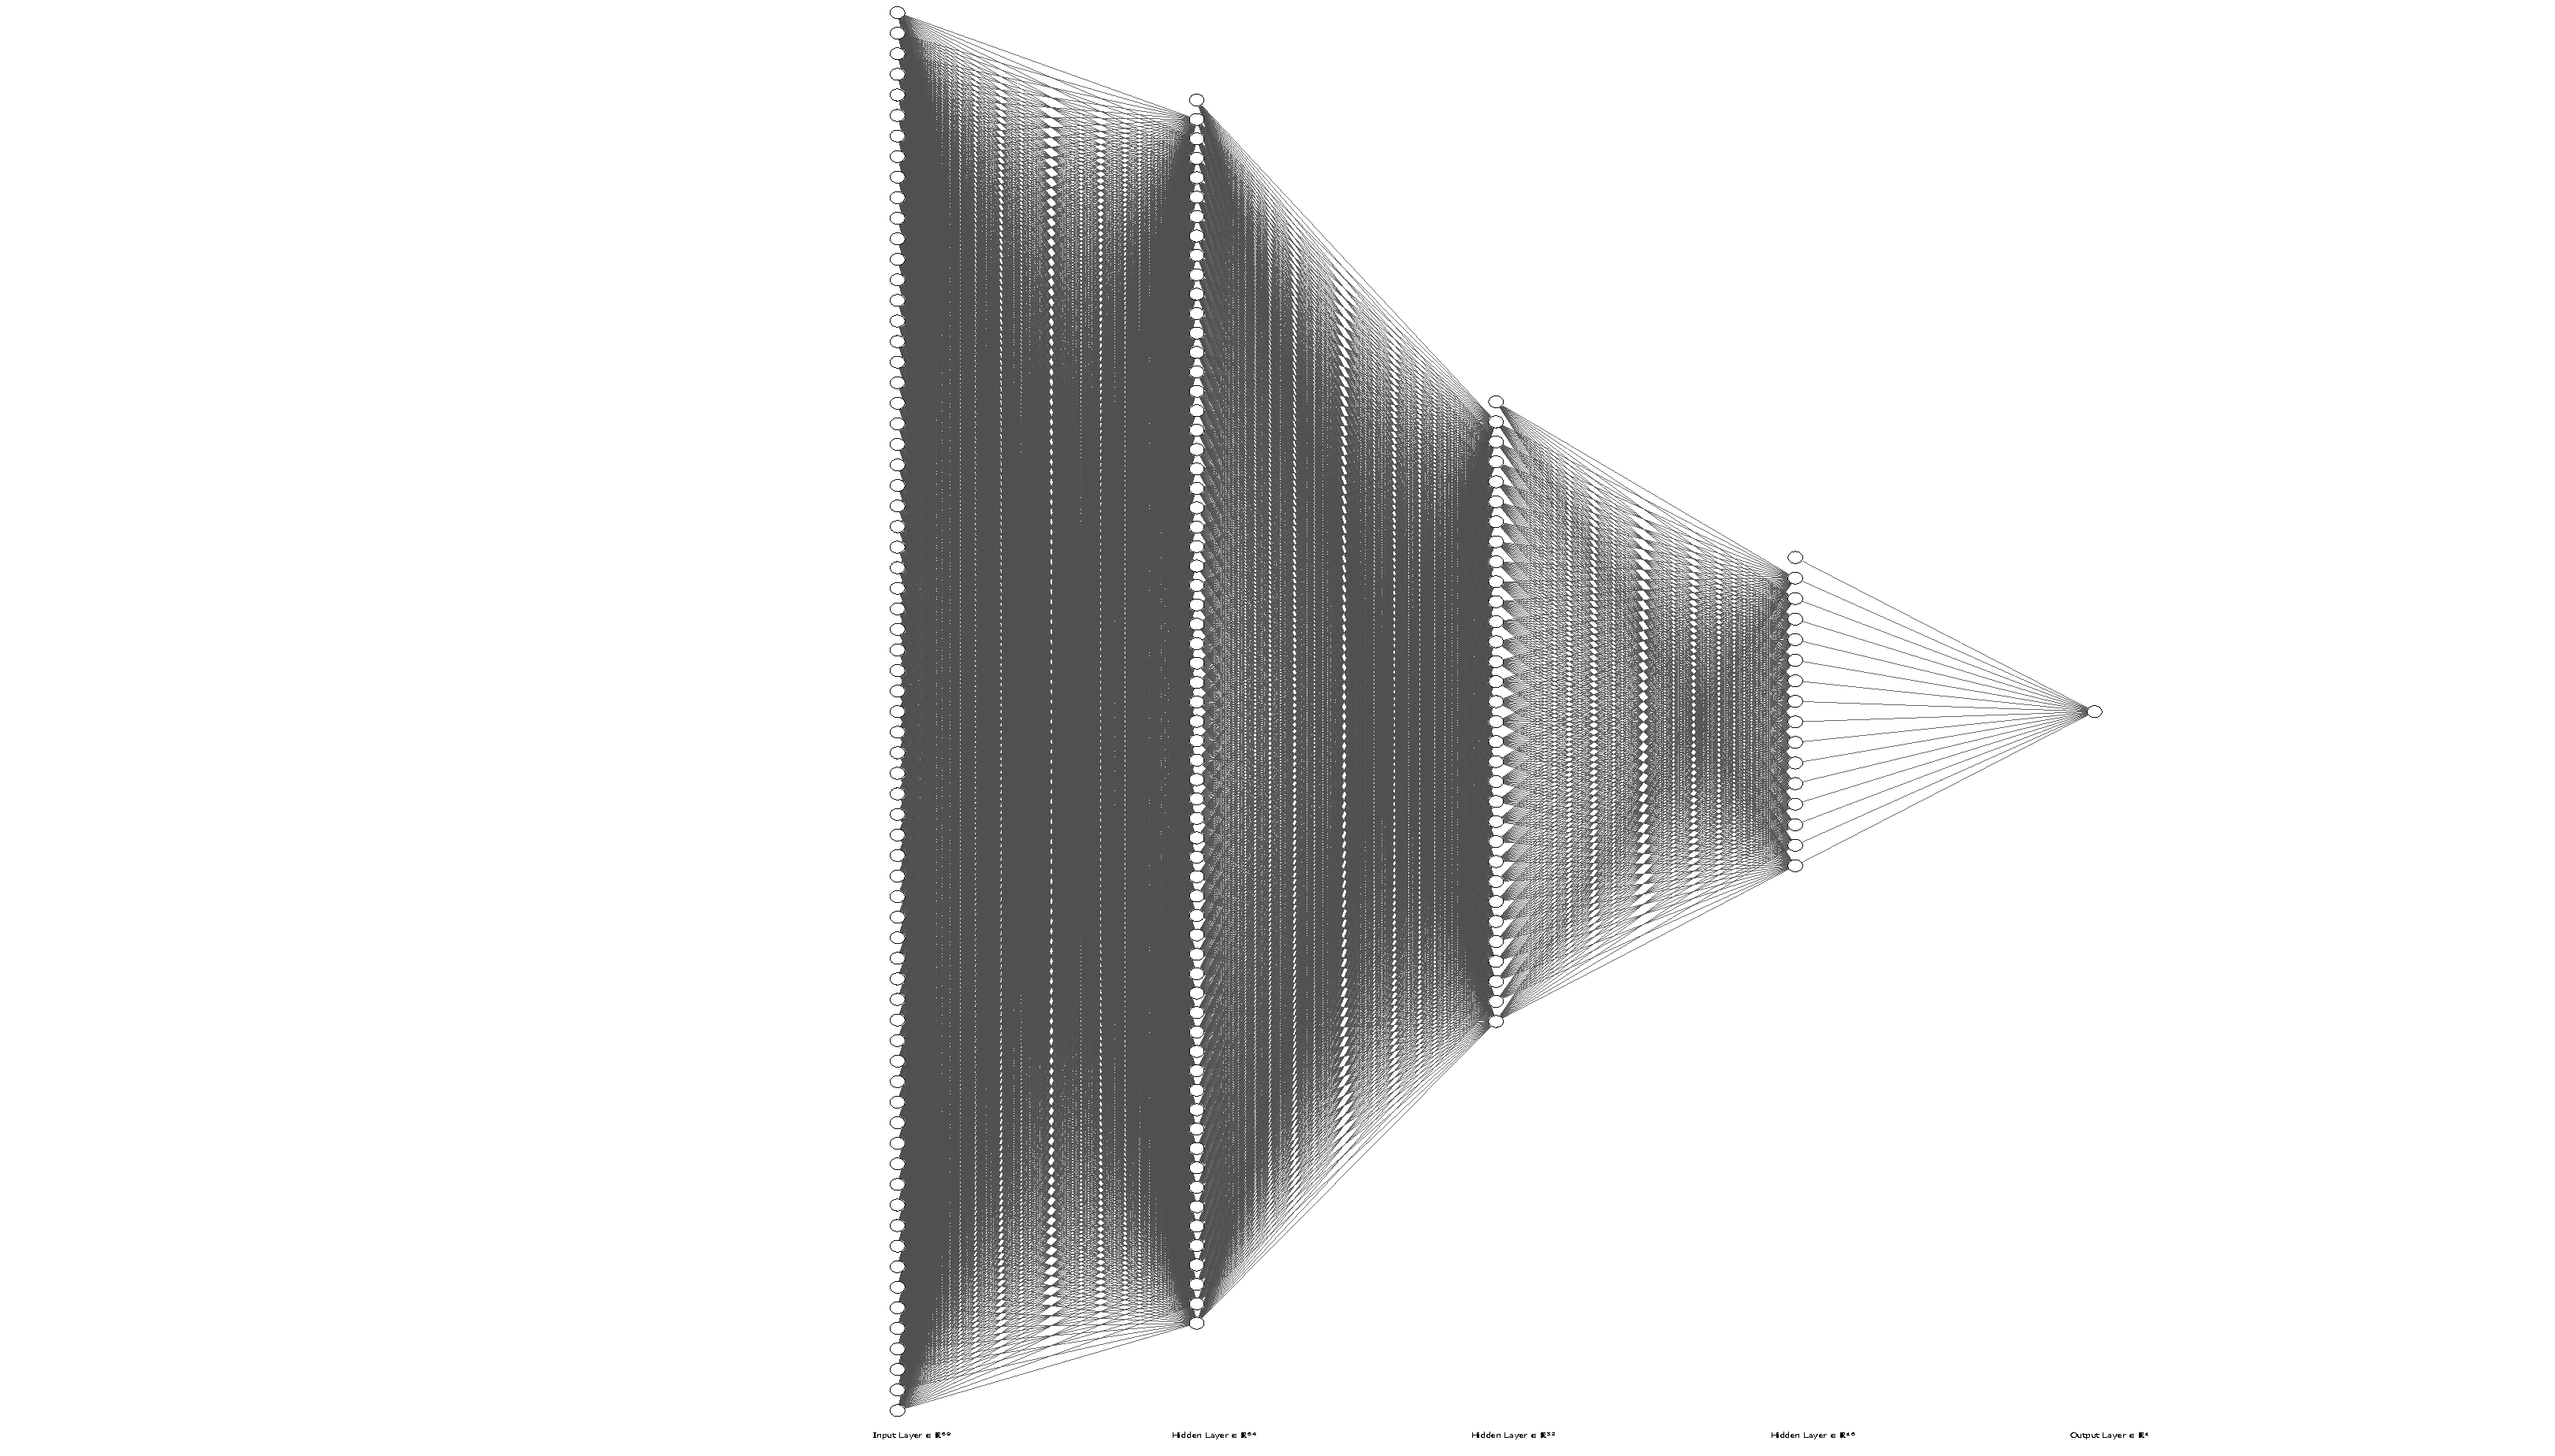
\includegraphics[width=0.5\textwidth]{figs/nn.pdf}
    \caption{DNN 结构示意图}
    \label{{fig:DNN}}
  \end{figure}
\end{enumerate}

\subsubsection{特征维度}
我在进行特征提取时得到的各个特征的维度分别为:
  \begin{itemize}
    \item \emph{短时能量}:$1$
    \item \emph{短时过零率}:$1$
    \item \emph{短时基频}:$1$
    \item \emph{短时频谱中心}:$1$
    \item \emph{短时子带能量}:$6$
    \item \emph{FBanks}:$23$
    \item \emph{MFCC}:$12$
    \item \emph{Delta MFCC}:$12$
    \item \emph{Delta of Delta MFCC}:$12$
  \end{itemize}
  因此,输入维度为$69$

\subsection{实验结果}

\subsubsection{各项性能表征}
在本次作业中,我主要考虑的参数是帧长与帧移,我训练数据集\emph{train}中的语音逐帧提取出特征与标签后,
按帧全部拼接到一起,然后进行训练集和验证集$4: 1$的划分,然后尝试使用不同的帧长帧移组合,训练\emph{DNN},
同时观察在验证集上的性能,最后考量其在开发集\emph{dev}上的各项性能,得到下表\ref{tab:DNN}中的数据以及对应的\emph{ROC}曲线(图\ref{fig:ROC DNN})

\begin{table*}[ht]
  \caption{DNN 分类效果}
  \label{tab:DNN}
  \centering
  \begin{tabular}{c|c|c|c|c|c|c|c|c}
    \toprule
    \textbf{Frame Length} & \textbf{Frame Shift} & \textbf{Loss} & \textbf{AUC} & \textbf{EER} & \textbf{Accuracy} & \textbf{Precision} & \textbf{Recall} & \textbf{F1 Score}\\
    \midrule
    320 & 80  & 0.1534 & 0.9832 & 0.0558 & 0.9500 & 0.9782 & 0.9602 & 0.9691 \\
    512 & 128 & 0.1491 & 0.9876 & 0.0464 & 0.9603 & 0.9765 & 0.9749 & 0.9757 \\
    1024 & 256 & 0.1277 & 0.9923 & 0.0376 & 0.9702 & 0.9755 & 0.9884 & 0.9819 \\
    2048 & 512 & 0.1351 & 0.9933 & \textbf{0.0319} & 0.9742 & 0.9803 & 0.9885 & 0.9844 \\
    4096 & 1024 & 0.1627 & 0.9913 & 0.0351 & 0.9722 & 0.9762 & \textbf{0.9905} & 0.9833 \\
    320 & 160 & 0.1655 & 0.9880 & 0.0447 & 0.9589 & 0.9701 & 0.9800 & 0.9750 \\
    512 & 256 & 0.1283 & 0.9917 & 0.0388 & 0.9687 & 0.9750 & 0.9869 & 0.9809 \\
    1024 & 512 & \textbf{0.1122} & 0.9934 & 0.0350 & 0.9742 & 0.9794 & 0.9893 & 0.9843 \\
    2048 & 1024 & 0.1182 & \textbf{0.9936} & 0.0332 & \textbf{0.9754} & \textbf{0.9834} & 0.9865 & \textbf{0.9849} \\
    4096 & 2048 & 0.1607 & 0.9901 & 0.0391 & 0.9722 & 0.9796 & 0.9865 & 0.9831 \\
    \bottomrule
  \end{tabular}
\end{table*}

\begin{figure}[ht]
  \centering
  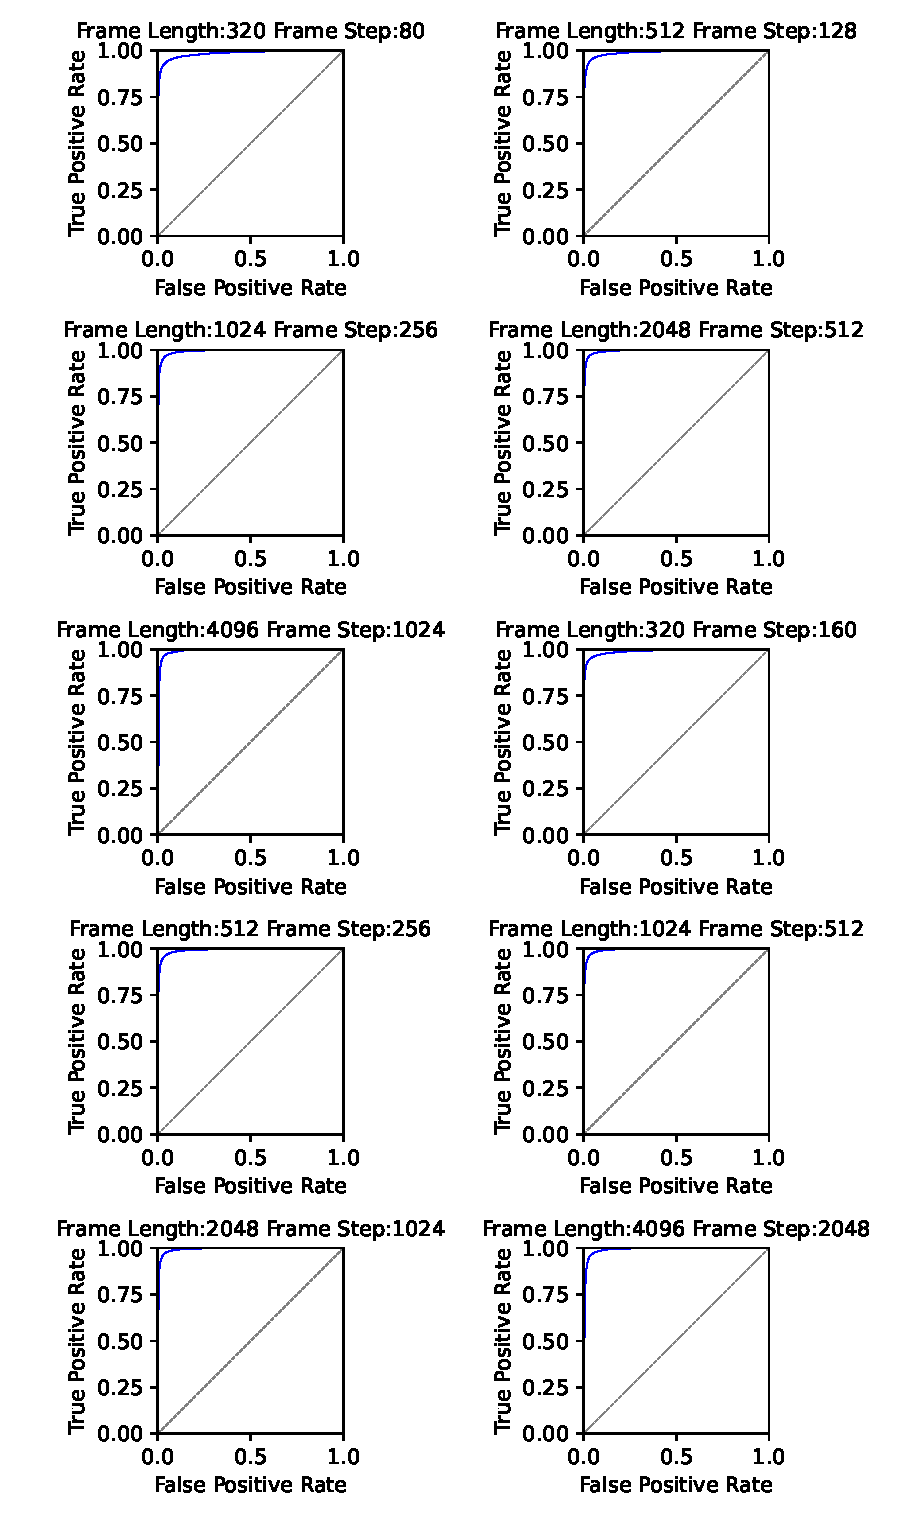
\includegraphics[width=0.5\textwidth]{figs/ROC_DNN.pdf}
  \caption{不同分帧方法下使用\emph{DNN}的\emph{ROC}曲线}
  \label{fig:ROC DNN}
\end{figure}
通过观察可以发现,\emph{DNN}的二分类性能均会随着帧长的增加而提升,
但是这仅仅说明模型对切分好的帧有较强的分类能力,于是我进行了如下时域信号切分的可视化。

\subsubsection{可视化}
随后,我取出了开发集中的一段语音信号,并使用不同分帧方法,测试了\emph{DNN}的表现,
得到如图\ref{fig:results DNN}中的效果。
\begin{figure}[ht]
  \centering
  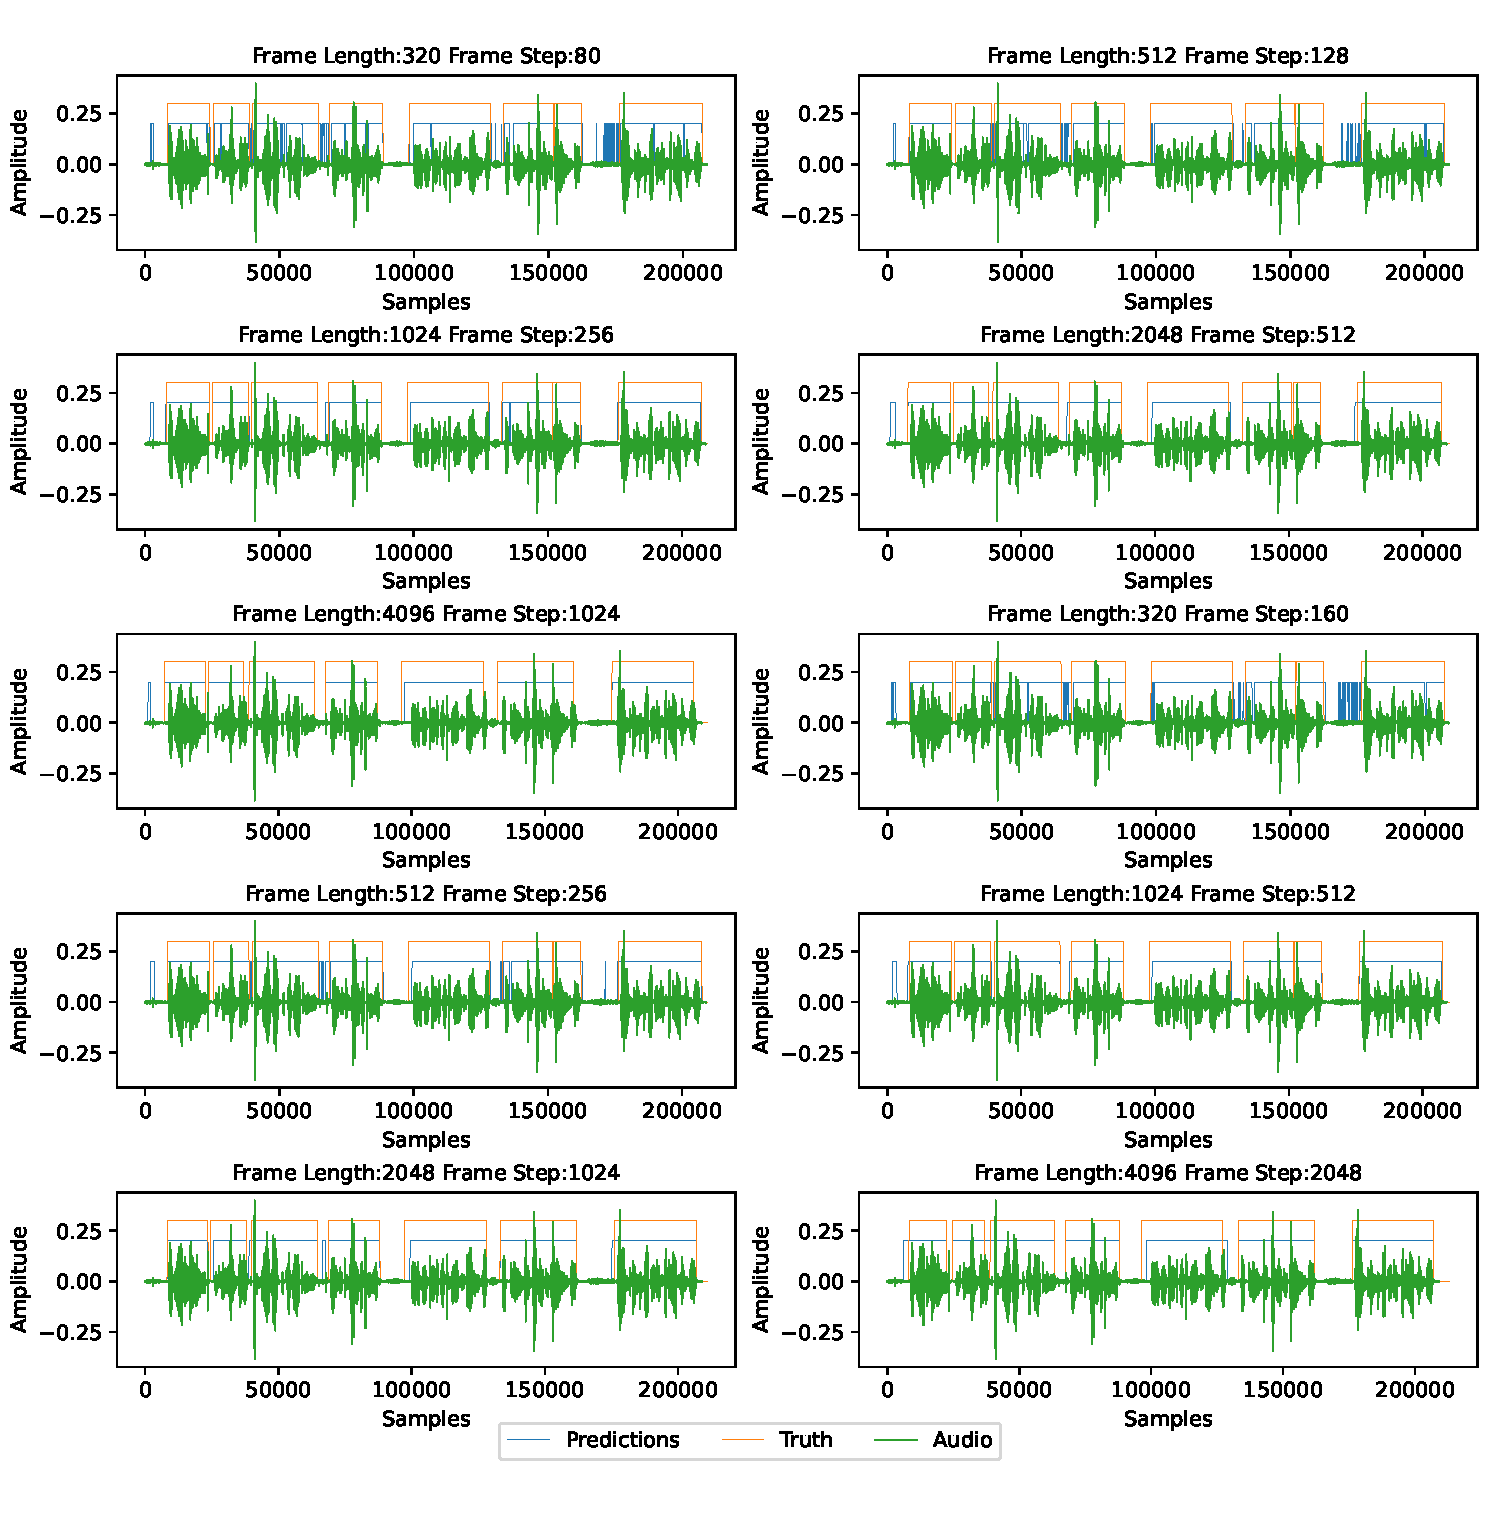
\includegraphics[width=0.5\textwidth]{figs/visualize_results_DNN.pdf}
  \caption{不同分帧方法下使用\emph{DNN}的表现}
  \label{fig:results DNN}
\end{figure}

可以看出,相较于简答的线性分类模型,\emph{DNN}的划分效果是更好的。
而且同样的,在帧长和帧移都比较小的时候,划分是更加精细的,但是会存在较多的非语音片段被划分为语音片段的情况,
相比之下,在帧长较大时,划分可能更粗犷,但是上述错误会少很多。

综合考虑,最后的结果我将使用\emph{帧长$4096$}和\emph{帧移$1024$}来进行分帧。

\section{一些思考}
\subsection{本次实验中的不足之处}
\begin{itemize}
  \item 在本次实验中,很多预处理操作,特征提取以及后期平滑操作等,都有很多参数可以调整,
  由于计算资源有限,在两次实验中我仅仅进行了关于帧长和帧移这两组参数的对比试验
  \item 在任务一中,我尝试过使用设置各个特征的阈值,来进行“硬”’分类,
  虽然\emph{Accuracy},\emph{Precision}等都表现不错,但是\emph{AUC}以及\emph{EER}指标就失去了其参考价值,
  因此不在报告中给出
  \item 在任务二中,我之前使用过自己写的\emph{GMM}分类器,但是性能比较差,
  后面我又尝试直接调用了\emph{sklearn}中的\emph{GMM},但是和我自己的\emph{GMM}一样,性能较差,
  不论是否进行数据特征归一化,在不同帧长组合上\emph{Accuracy}都只有$80\%$左右,
  这可能与我提取的特征有直接关系,导致出现了老师上课讲的\emph{极大似然}可能效果较差的情况,因此不在报告中给出
\end{itemize}

\subsection{关于AI的使用情况}
\begin{itemize}
  \item 在实验部分,最底层的框架以及大部分实验代码均是本人完成的,在涉及某些复杂的或者课内没有讲过的特征提取和处理时,
  我会先去询问Chat GPT,然后尽可能自己复现
  \item 在报告书写时,在很多特征和处理的描述方面,我可能做不到精确缜密的组织语言,因此我会先去咨询Chat GPT,然后组织好语言加进报告中
\end{itemize}

\subsection{关于VAD性能指标的思考}
\begin{itemize}
  \item 使用逐帧的二分类指标来衡量一个VAD模型的好坏是否恰当?这样能否表征语音的动态特性?
  \item 从图\ref{fig:results Linear SVM},图\ref{fig:results Logistic Regression}以及图\ref{fig:results DNN}中其实不难发现,
  在一段语音信号的边界处,模型的预测并不能完全同真实标注契合,这是否可以通过论文\href{https://ieeexplore.ieee.org/document/7015406}{Evaluating vad for automatic speech recognition}
  中提出的\emph{起始边界准确率(SBA)}和\emph{结束边界准确率(EBA)}来刻画?
  \item 在帧长比较小时,模型的预测可能比较跳跃,将一大段语音信号切分成了很多小段,输出很多没必要的划分,这能否通过上面文章中的\emph{边界精确率(BP)}来刻画?
\end{itemize}



\end{document}
